\chapter{Les nombres entiers}
{https://sacado.xyz/qcm/parcours_show_course/0/117118}
{


 \begin{CpsCol}
\textbf{Les savoir-faire du parcours} 
 \begin{itemize}
 \item Savoir écrire un nombre entier en lettres.
 \item Savoir écrire un nombre entier en chiffres.
 \item Savoir déterminer la valeur d'un chiffre selon sa position.
 \item Savoir déterminer un nombre de ... dans un nombre entier.
 \item Savoir décomposer un nombre entier.
 \item Savoir comparer des nombres entiers.
 \item Savoir encadrer un nombre entier.
 \item Savoir repérer un nombre entier sur une demi-droite graduée.
 \item Savoir placer un nombre sur une demi-droite graduée.
 \end{itemize}
 \end{CpsCol}

}

\begin{pageCours} 


\section{Nombres entiers}

\begin{Def}
Un \textbf{nombre entier} est un nombre qui peut s'écrire \textbf{sans virgule}
\end{Def}

\begin{Rqs}
\begin{itemize}
\item $0$, $1$, $2$, $3$, $4$, $5$, $6$, $7$, $8$ et $9$ sont les dix \textbf{chiffres} qui permettent d'écrire tous les nombres entiers.
\item Pour pouvoir lire les grands nombres entiers facilement, on regroupe les chiffres par groupe de 3 : $345\,202$
\end{itemize}
\end{Rqs}

\begin{Reg}
Règles orthographiques pour l'écriture des nombres :
\begin{itemize}[leftmargin=*]
    \item Un trait d'union entre chaque mot.
    \item Les mots servant à écrire les nombres sont tous invariable sauf :
    \begin{itemize}
        \item Au pluriel million et milliard prennent un 's'.
        \item Au pluriel cent et vingt prennent un 's' lorsqu'ils ne sont pas suivi par un autre nombre.
    \end{itemize}
\end{itemize}
\end{Reg}



\section{Position d'un chiffre dans un nombre}

\begin{Def}
\begin{itemize}[leftmargin=*]
\item Notre système numérique est un \textbf{système décimal} (numération décimale).
\item Chaque \textbf{chiffre} à une valeur en fonction de sa \textbf{position} dans le nombre (numération de position)
\end{itemize}
\end{Def}

\begin{Ex}
Un million = $1\,000\,000$ unités
\end{Ex}

\begin{VocU}

\begin{minipage}{0.3\linewidth}

Chaque position (rang) possède un nom spécifique : unité, dizaine, centaines....

\end{minipage}
\begin{minipage}{0.7\linewidth}

 \begin{tabular}{|c|c c|c c|c|c|c|c|c|c|c|}
   \hline \rowcolor{sacado_green!10!white}
      \rotatebox[origin=c]{90}{Millions} & \rotatebox[origin=c]{90}{Centaines }  & \rotatebox[origin=c]{90}{ de milliers}  &\rotatebox[origin=c]{90}{Dizaines }&\rotatebox[origin=c]{90}{  de milliers} & \rotatebox[origin=c]{90}{Milliers} & \rotatebox[origin=c]{90}{Centaines} & \rotatebox[origin=c]{90}{Dizaines} & \rotatebox[origin=c]{90}{Unités} & \rotatebox[origin=c]{90}{Dixièmes} & \rotatebox[origin=c]{90}{Centièmes} & \rotatebox[origin=c]{90}{Millièmes} \rule[-7pt]{0pt}{20pt} \\  \hline
 
    & &{\LARGE 9 }&   & {\LARGE 8 } &{\LARGE 4  } & {\LARGE 6 } & {\LARGE 1 }  & {\LARGE 2, }  & {\LARGE 3 }  &  {\LARGE 7} & {\LARGE 5} \\ 
   \hline 
   \end{tabular}   
   
\end{minipage}    
 
\end{VocU}

\begin{MtT}{Décomposition décimale d'un nombre.}
 $437\,640\,881$ se décompose sous les forme : \index{Décomposition décimale}
\begin{itemize}[leftmargin=*]
\item Décomposition 1 : $437\,000\,000+640\,000+881$
\item Décomposition 2 : $(437\times1\,000\,000)+(640\times 1\,000)+(881\times1)$
\item Décomposition 3 : $400\,000\,000+30\,000\,000+7\,000\,000+600\,000+40\,000+800+80+1$
\item Décomposition 4 : $4\times100\,000\,000+3\times10\,000\,000+7\times1\,000\,000+6\times100\,000+4\times10\,000+8\times100+8\times10+1\times1$
\end{itemize}
\end{MtT}



\end{pageCours} 

\begin{pageAD} 


\Sf{ Savoir écrire un nombre entier en lettres.} 

% ExoCad 7 paramètres : Compétences, qrcode , calculatrice, python, scratch, tableur, annales
\begin{ExoCad}{Chercher. Représenter.}{1234}{2}{0}{0}{0}{0}

Écris les nombres donnés en lettres 

\begin{itemize}[leftmargin=*]
\item $2\,435$ s'écrit :\point{1} 
\item $146\,234$ s'écrit : \point{1} 
\item $1\,768\,255$ s'écrit :\point{1} 
\end{itemize}

\end{ExoCad}
 
 \Sf{ Savoir écrire un nombre entier en chiffres.}
 
 \begin{ExoCad}{Chercher. Représenter.}{1234}{2}{0}{0}{0}{0}
 \begin{itemize}[leftmargin=*]
\item Cent-dix-huit-mille-quarante-trois s'écrit :\point{1} 
\item Trois-mille-deux-cent-quatre-vingt-cing s'écrit : \point{1} 
\item Deux-millions-quatre-cent-douze-mille-six-cent-quinze s'écrit :\point{1} 
\end{itemize}
  \end{ExoCad}
  
 \begin{ExoCad}{Chercher. Représenter.}{1234}{1}{0}{0}{0}{0}
 
Complète la phrase suivante en écrivant le nombre rouge en chiffres :

« Au mois de juin 2018, la population mondiale est d’environ {\color{sacado_red}sept-milliards-cinq-cent
cinquante-neuf-millions-deux-cent-quatre-vingt-huit-mille-trois-cents}  personnes. »

$\ldots\ldots\ldots\ldots\ldots\ldots\ldots\ldots\ldots\ldots$
  \end{ExoCad} 
  
  
 \Sf{ Savoir déterminer la valeur d'un chiffre selon sa position.}
 
  
\begin{ExoCad}{Chercher. Représenter.}{1234}{1}{0}{0}{0}{0}
 
\begin{enumerate}[leftmargin=*]
\item Dans le nombre $245\,691$, quel est le chiffre des centaines ? \point{1}  
\item Dans le nombre $142\,360\,758$, quel est le chiffre des dizaines de millier ?\point{1} 
\item Dans le nombre $3\,298\,731$, quel est le chiffre des milliers ?\point{1}
\end{enumerate} 


\end{ExoCad} 
  
 
\Sf{ Savoir déterminer un nombre de ... dans un nombre entier.}
 
 
\begin{ExoCad}{Chercher. Représenter.}{1234}{1}{0}{0}{0}{0}
 
\begin{enumerate}[leftmargin=*]
\item Combien de centaines le nombre $235\,142$ compte-il ? \point{1}
\item Combien de milliers le nombre $605\,404$ compte-il ?\point{1}
\item Combien de dizaines le nombre $14\,405$ compte-il ?\point{1}
\end{enumerate} 
\end{ExoCad}
  
\Sf{ Savoir décomposer un nombre entier.}
 
\begin{ExoCad}{Chercher. Représenter.}{1234}{2}{0}{0}{0}{0}
 
 Décompose les nombres :
 
\begin{itemize}[leftmargin=*]
\item $340\,324 = \ldots\ldots \times 100\,000+\ldots\ldots \times 10\,000+\ldots\ldots \times 1\,000+\ldots\ldots \times 100+\ldots\ldots \times 10+\ldots\ldots$
\item $92\,051 = \ldots\ldots \times 10\,000+\ldots\ldots \times 1\,000+\ldots\ldots \times 100+\ldots\ldots \times 10+\ldots\ldots$
\end{itemize} 

\end{ExoCad}




\end{pageAD} 


\begin{pageCours}
 
\section{Comparer des nombres entiers}

\begin{DefT}{Comparer}  

\textbf{Comparer}\index{Comparer|Nombres} deux nombres, c'est trouver le \textbf{plus grand} (ou le \textbf{plus petit}) ou dire s'ils sont \textbf{égaux}.

On utilise les \textbf{symboles de comparaison} :
\begin{center}
"est \textbf{supérieur} à" ($>$) , "est \textbf{inférieur} à" ($<$), "est \textbf{égal} à" ($=$)
\end{center}
\end{DefT}

\begin{Ex}
$29\,874\,492$ est {\color{sacado_orange!80}supérieur à } $27\,514\,420$ donc $29\,874\,492 {\color{sacado_orange!80}>} 27\,514\,420$.
\end{Ex}

 

\begin{DefT}{Ordre}\index{Ordre croissant}\index{Ordre décroissant}
\begin{itemize}[leftmargin=*]
\item Ranger des nombres dans \textbf{l'ordre croissant} signifie les ranger \textbf{du plus petit au plus grand}.
\item Ranger des nombres dans \textbf{l'ordre décroissant} signifie les ranger \textbf{du plus grand au plus petit}.
\end{itemize}
\end{DefT}



\section{Encadrer un nombre entier}

\begin{DefT}{Encadrer un nombre}
\textbf{Encadrer}\index{Encadrer|Nombres} un nombre, c'est trouver un nombre plus petit et un nombre plus grand.

La \textbf{précision de l'encadrement}\index{Précision|Nombres} est la \textbf{différence} entre les deux nombres trouvés.
\end{DefT}

\begin{Ex}
Encadrement du nombre $143\,526$ :

à la {\color{sacado_blue}dizaine} : \(143\,5{\color{sacado_blue!80!black}2}0 < 143\,5{\color{sacado_blue!80!black}2}6 < 143\,5{\color{sacado_blue!80!black}3}0\) \quad à la {\color{sacado_orange!80!black}centaine} : \(143\,{\color{sacado_orange!80!black}5}00 < 143\,{\color{sacado_orange!80!black}5}26 < 143\,{\color{sacado_orange!80!black}6}00\)
\end{Ex}
 


\section{Nombres entiers et demi-droite graduée}

\begin{DefT}{demi-droite graduée}

Une \textbf{demi-droite graduée}\index{demi-droite graduée} est une \textbf{demi-droite} sur laquelle on a reporté une \textbf{unité de longueur} régulièrement à partir de son \textbf{origine}. L'origine est repérée par le nombre $0$.

Sur une demi-droite graduée, \textbf{un point} est repéré par \textbf{un nombre}, son \textbf{abscisse}\index{abscisse}.


\begin{center}
\begin{tikzpicture}[line cap=round,line join=round,>=triangle 45,x=1.0cm,y=1.0cm]
\begin{axis}[
x=1.0cm,y=1.0cm,
axis lines=middle,
xmin=0,
xmax=9.640000000000004,
ymin=-0.199999999999999,
ymax=0.0199999999999998,
xtick={-0.0,1.0,...,9.0},
ytick={-0.0,1.0,...,1.0},]
\clip(-0.7,-0.62) rectangle (9.64,1.02);
\draw (0.14,-0.54) node {$0$};
\begin{scriptsize}
\draw [color=xdxdff] (4.,0.)-- ++(-2.5pt,0 pt) -- ++(5.0pt,0 pt) ++(-2.5pt,-2.5pt) -- ++(0 pt,5.0pt);
\draw[color=xdxdff] (4.14,0.37) node {$A$};
\end{scriptsize}
\end{axis}
\end{tikzpicture}
\end{center}

\end{DefT}

\end{pageCours} 

\begin{pageAD} 
 

\Sf{ Savoir comparer des nombres entiers.}
 
\begin{ExoCad}{Chercher. Représenter.}{1234}{2}{0}{0}{0}{0}

 Complète avec > , < ou = :
 
 \begin{minipage}{0.3\linewidth}
  \[567 \ldots\ldots 455\]
  \[23\,717 \ldots\ldots 23\,177 \]
  \[91\,456\,022 \ldots\ldots 83\,427\,923\]
  \end{minipage}\hfill
 \begin{minipage}{0.3\linewidth}
  \[10\,047 \ldots\ldots 1\,047 \]
  \[49\,017 \ldots\ldots 50\,077 \]
  \[99\,537\,152 \ldots\ldots 99\,537\,152 \]
  \end{minipage}
  \hfill
 \begin{minipage}{0.3\linewidth}
  \[23\,047 \ldots\ldots 23\,047 \]
  \[19\,003 \ldots\ldots 99\,003 \]
  \[104\,004\,576  \ldots\ldots 104\,004\,567 \]
  \end{minipage}  
  
\end{ExoCad} 
  
  
\begin{ExoCad}{Chercher. Représenter.}{1234}{2}{0}{0}{0}{0}
 
\begin{enumerate}[leftmargin=*]
 \item Mettre les nombres suivants dans l'ordre croissant : $93\,692 \hspace{.5cm} 83\,321 \hspace{.5cm} 44\,512 \hspace{.5cm} 65\,173$ 
 
 \point{1}
 \item Mettre les nombres suivants dans l'ordre décroissant : $7\,096 \hspace{.5cm} 8\,623 \hspace{.5cm} 56\,393 \hspace{.5cm} 13\,582$	
 
 \point{1}	
\end{enumerate}
\end{ExoCad} 
 
\Sf{ Savoir encadrer un nombre entier.}


\begin{ExoCad}{Chercher. Représenter.}{1234}{2}{0}{0}{0}{0}
\begin{enumerate}[leftmargin=*]  
\item Encadrer le nombre $33\,409$ à la \textbf{centaine} près. \point{1}
\item Encadrer le nombre $19\,322$ à la \textbf{dizaine} près. \point{1} 
\item Encadrer le nombre $14\,995$ au \textbf{millier} près. \point{1} 
\end{enumerate}
\end{ExoCad}
    
 


 
 \Sf{ Savoir repérer un nombre entier sur une demi-droite graduée.}
 
 
\begin{ExoCad}{Chercher. Représenter.}{1234}{2}{0}{0}{0}{0}

Sur la droite graduée, placer 

\begin{enumerate}[leftmargin=*]  
\item le point $A$ d'abscisse $4$.
\item le point $B$ d'abscisse $8$.
\item le point $C$ d'abscisse $2$.
\end{enumerate}
 
 
\definecolor{qqqqff}{rgb}{0.,0.,1.}
\definecolor{xdxdff}{rgb}{0.49019607843137253,0.49019607843137253,1.}
\definecolor{ududff}{rgb}{0.30196078431372547,0.30196078431372547,1.}
\definecolor{cqcqcq}{rgb}{0.7529411764705882,0.7529411764705882,0.7529411764705882}
\begin{tikzpicture}[line cap=round,line join=round,>=triangle 45,x=1.0cm,y=1.0cm]
\clip(-2.7075152359835273,2.3774601565681697) rectangle (11.562491953884278,3.6234089425866403);
\draw [line width=2.pt,color=ududff] (-2.,3.)-- (11.,3.);
\draw [color=qqqqff](-2.162412642100446,3.) node[anchor=north west] {$0$};
\draw [color=qqqqff](-1.1695472032419765,3.) node[anchor=north west] {$1$};
\begin{scriptsize}
\draw [color=ududff] (-2.,3.)-- ++(-2.5pt,0 pt) -- ++(5.0pt,0 pt) ++(-2.5pt,-2.5pt) -- ++(0 pt,5.0pt);
\draw [color=xdxdff] (-1.,3.)-- ++(-2.5pt,0 pt) -- ++(5.0pt,0 pt) ++(-2.5pt,-2.5pt) -- ++(0 pt,5.0pt);
\draw [color=xdxdff] (0.,3.)-- ++(-2.5pt,0 pt) -- ++(5.0pt,0 pt) ++(-2.5pt,-2.5pt) -- ++(0 pt,5.0pt);
\draw [color=ududff] (1.,3.)-- ++(-2.5pt,0 pt) -- ++(5.0pt,0 pt) ++(-2.5pt,-2.5pt) -- ++(0 pt,5.0pt);
\draw [color=ududff] (2.,3.)-- ++(-2.5pt,0 pt) -- ++(5.0pt,0 pt) ++(-2.5pt,-2.5pt) -- ++(0 pt,5.0pt);
\draw [color=xdxdff] (3.,3.)-- ++(-2.5pt,0 pt) -- ++(5.0pt,0 pt) ++(-2.5pt,-2.5pt) -- ++(0 pt,5.0pt);
\draw [color=xdxdff] (4.,3.)-- ++(-2.5pt,0 pt) -- ++(5.0pt,0 pt) ++(-2.5pt,-2.5pt) -- ++(0 pt,5.0pt);
\draw [color=xdxdff] (5.,3.)-- ++(-2.5pt,0 pt) -- ++(5.0pt,0 pt) ++(-2.5pt,-2.5pt) -- ++(0 pt,5.0pt);
\draw [color=xdxdff] (6.,3.)-- ++(-2.5pt,0 pt) -- ++(5.0pt,0 pt) ++(-2.5pt,-2.5pt) -- ++(0 pt,5.0pt);
\draw [color=xdxdff] (7.,3.)-- ++(-2.5pt,0 pt) -- ++(5.0pt,0 pt) ++(-2.5pt,-2.5pt) -- ++(0 pt,5.0pt);
\draw [color=xdxdff] (8.,3.)-- ++(-2.5pt,0 pt) -- ++(5.0pt,0 pt) ++(-2.5pt,-2.5pt) -- ++(0 pt,5.0pt);
\draw [color=xdxdff] (9.,3.)-- ++(-2.5pt,0 pt) -- ++(5.0pt,0 pt) ++(-2.5pt,-2.5pt) -- ++(0 pt,5.0pt);
\draw [color=xdxdff] (10.,3.)-- ++(-2.5pt,0 pt) -- ++(5.0pt,0 pt) ++(-2.5pt,-2.5pt) -- ++(0 pt,5.0pt);
\end{scriptsize}
\end{tikzpicture}
 
 
\end{ExoCad}
    
\begin{ExoCad}{Chercher. Représenter.}{1234}{2}{0}{0}{0}{0}
 
 \definecolor{qqqqff}{rgb}{0.,0.,1.}
\definecolor{ffqqqq}{rgb}{1.,0.,0.}
\definecolor{xdxdff}{rgb}{0.49019607843137253,0.49019607843137253,1.}
\definecolor{ududff}{rgb}{0.30196078431372547,0.30196078431372547,1.}
\begin{tikzpicture}[line cap=round,line join=round,>=triangle 45,x=1.0cm,y=1.0cm]
\clip(-2.376560089697371,2.260652457878938) rectangle (11.251004757379661,3.895960239528181);
\draw [line width=2.pt,color=ududff] (-2.,3.)-- (11.,3.);
\draw [color=qqqqff](-2.162412642100446,2.9) node[anchor=north west] {$0$};
\draw [color=qqqqff](7.649434047795016,2.9) node[anchor=north west] {$100$};
\draw [color=ffqqqq](0.6993759757857307,3.527) node[anchor=north west] {$A$};
\draw [color=ffqqqq](6.75390835784424,3.527) node[anchor=north west] {$B$};
\begin{scriptsize}
\draw [color=ududff] (-2.,3.)-- ++(-2.5pt,0 pt) -- ++(5.0pt,0 pt) ++(-2.5pt,-2.5pt) -- ++(0 pt,5.0pt);
\draw [color=xdxdff] (-1.,3.)-- ++(-2.5pt,0 pt) -- ++(5.0pt,0 pt) ++(-2.5pt,-2.5pt) -- ++(0 pt,5.0pt);
\draw [color=xdxdff] (0.,3.)-- ++(-2.5pt,0 pt) -- ++(5.0pt,0 pt) ++(-2.5pt,-2.5pt) -- ++(0 pt,5.0pt);
\draw [color=ffqqqq] (1.,3.)-- ++(-2.5pt,0 pt) -- ++(5.0pt,0 pt) ++(-2.5pt,-2.5pt) -- ++(0 pt,5.0pt);
\draw [color=ududff] (2.,3.)-- ++(-2.5pt,0 pt) -- ++(5.0pt,0 pt) ++(-2.5pt,-2.5pt) -- ++(0 pt,5.0pt);
\draw [color=xdxdff] (3.,3.)-- ++(-2.5pt,0 pt) -- ++(5.0pt,0 pt) ++(-2.5pt,-2.5pt) -- ++(0 pt,5.0pt);
\draw [color=xdxdff] (4.,3.)-- ++(-2.5pt,0 pt) -- ++(5.0pt,0 pt) ++(-2.5pt,-2.5pt) -- ++(0 pt,5.0pt);
\draw [color=xdxdff] (5.,3.)-- ++(-2.5pt,0 pt) -- ++(5.0pt,0 pt) ++(-2.5pt,-2.5pt) -- ++(0 pt,5.0pt);
\draw [color=xdxdff] (6.,3.)-- ++(-2.5pt,0 pt) -- ++(5.0pt,0 pt) ++(-2.5pt,-2.5pt) -- ++(0 pt,5.0pt);
\draw [color=ffqqqq] (7.,3.)-- ++(-2.5pt,0 pt) -- ++(5.0pt,0 pt) ++(-2.5pt,-2.5pt) -- ++(0 pt,5.0pt);
\draw [color=xdxdff] (8.,3.)-- ++(-2.5pt,0 pt) -- ++(5.0pt,0 pt) ++(-2.5pt,-2.5pt) -- ++(0 pt,5.0pt);
\draw [color=xdxdff] (9.,3.)-- ++(-2.5pt,0 pt) -- ++(5.0pt,0 pt) ++(-2.5pt,-2.5pt) -- ++(0 pt,5.0pt);
\draw [color=xdxdff] (10.,3.)-- ++(-2.5pt,0 pt) -- ++(5.0pt,0 pt) ++(-2.5pt,-2.5pt) -- ++(0 pt,5.0pt);
\end{scriptsize}
\end{tikzpicture}

\begin{enumerate}[leftmargin=*]  
\item Lire l'abscisse du point $A$ \point{1}
\item Lire l'abscisse du point $B$ \point{1}
\end{enumerate}


\end{ExoCad}
    
\begin{ExoCad}{Chercher. Représenter.}{1234}{2}{0}{0}{0}{0}

Je suis un nombre entier compris entre  $98\,998$ et $99\,000$. Je suis $\ldots \ldots\ldots$

\end{ExoCad}
    
 

\end{pageAD} 


\begin{pageParcoursu}

\begin{ExoCu}{Représenter. Communiquer.}{1234}{2}{0}{0}{0}{0}

Écris en chiffres le nombre trente-cinq-mille-trente-sept : \point{1}
\vspace{0.2cm}
Écris en lettres le nombre $23\,506$ : \point{1}
  
\end{ExoCu}


% ExoCu 7 paramètres : Compétences, qrcode , calculatrice, python, scratch, tableur, annales
\begin{ExoCu}{Représenter.}{1234}{2}{0}{0}{0}{0}

Je suis le nombre entier compris entre  $98$ et $100$. Je suis \point{1} \vspace{0.2cm}
 
Je suis le nombre entier compris entre  $234\,980$ et $234\,982$. Je suis \point{1}
\end{ExoCu}

 % ExoCu 7 paramètres : Compétences, qrcode , calculatrice, python, scratch, tableur, annales
\begin{ExoCu}{Chercher. Représenter.}{1234}{2}{0}{0}{0}{0}

Détermine l'abscisse du point $M$ \point{1}

 %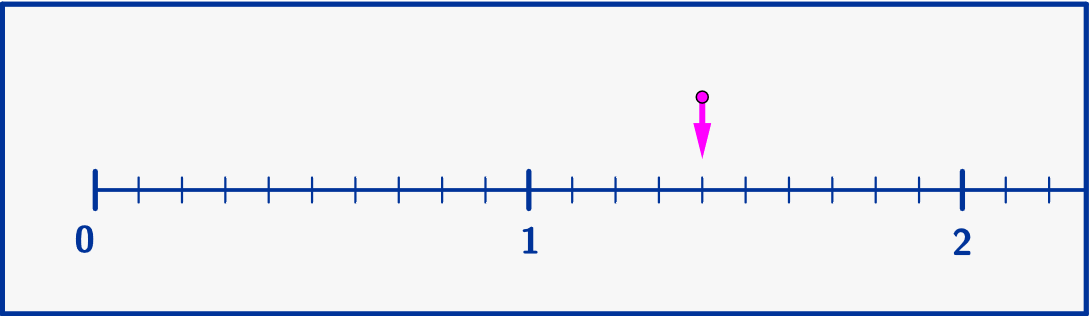
\includegraphics[width=.8\linewidth]{nombre_decimaux_demi-droite.png}
\begin{tikzpicture}[line cap=round,line join=round,>=triangle 45,x=.7cm,y=.7cm]
\clip(-7,-1.5) rectangle (11.5,2);
\fill[line width=1.2pt,color=eqeqeq,fill=eqeqeq,fill opacity=0.10000000149011612] (-6.5,2) -- (-6.5,-1.5) -- (11.,-1.5) -- (11.,2) -- cycle;
\draw[line width=1.4pt,color=qqzzff] (-3.038309699461245,4.543294499307796) -- (-1.9563840380590396,4.543294499307796);
\draw[line width=1.4pt,color=qqzzff] (-5.499690579151262,3.556818570075324) -- (-4.823487040774884,3.556818570075324);
\draw [line width=1.8pt,color=qqttzz] (-6.5,2.)-- (-6.5,-1.5);
\draw [line width=1.8pt,color=qqttzz] (-6.5,-1.5)-- (11.,-1.5);
\draw [line width=1.8pt,color=qqttzz] (11.,-1.5)-- (11.,2.);
\draw [line width=1.8pt,color=qqttzz] (11.,2.)-- (-6.5,2.);
\draw [line width=1.2pt,color=qqttzz] (-5.,-0.2)-- (-5.,0.2);
\draw [line width=1.2pt,color=qqttzz] (-4.3,-0.2)-- (-4.3,0.2);
\draw [line width=1.2pt,color=qqttzz] (-3.6,-0.2)-- (-3.6,0.2);
\draw [line width=1.2pt,color=qqttzz] (-2.9,-0.2)-- (-2.9,0.2);
\draw [line width=1.2pt,color=qqttzz] (-2.2,-0.2)-- (-2.2,0.2);
\draw [line width=1.2pt,color=qqttzz] (-1.5,-0.2)-- (-1.5,0.2);
\draw [line width=1.2pt,color=qqttzz] (-0.8,-0.2)-- (-0.8,0.2);
\draw [line width=1.2pt,color=qqttzz] (-0.1,-0.2)-- (-0.1,0.2);
\draw [line width=1.2pt,color=qqttzz] (0.6,-0.2)-- (0.6,0.2);
\draw [line width=1.2pt,color=qqttzz] (1.3,-0.2)-- (1.3,0.2);
\draw [line width=1.2pt,color=qqttzz] (2.,-0.2)-- (2.,0.2);
\draw [line width=1.2pt,color=qqttzz] (2.7,-0.2)-- (2.7,0.2);
\draw [line width=1.2pt,color=qqttzz] (3.4,-0.2)-- (3.4,0.2);
\draw [line width=1.2pt,color=qqttzz] (4.1,-0.2)-- (4.1,0.2);
\draw [line width=1.2pt,color=qqttzz] (4.8,-0.2)-- (4.8,0.2);
\draw [line width=1.2pt,color=qqttzz] (5.5,-0.2)-- (5.5,0.2);
\draw [line width=1.2pt,color=qqttzz] (6.2,-0.2)-- (6.2,0.2);
\draw [line width=1.2pt,color=qqttzz] (6.9,-0.2)-- (6.9,0.2);
\draw [line width=1.2pt,color=qqttzz] (7.6,-0.2)-- (7.6,0.2);
\draw [line width=1.2pt,color=qqttzz] (8.3,-0.2)-- (8.3,0.2);
\draw [line width=1.2pt,color=qqttzz] (9.,-0.2)-- (9.,0.2);
\draw [line width=1.2pt,color=qqttzz] (9.7,-0.2)-- (9.7,0.2);
\draw [line width=1.2pt,color=qqttzz] (10.4,-0.2)-- (10.4,0.2);
\draw [line width=1.8pt,color=qqttzz] (-5.,-0.3)-- (-5.,0.3);
\draw [line width=1.8pt,color=qqttzz] (2.,-0.3)-- (2.,0.3);
\draw [line width=1.8pt,color=qqttzz] (9.,-0.3)-- (9.,0.3);
\draw [->,line width=3.2pt,color=ffqqff] (4.8,1.5) -- (4.8,0.5);
\draw [line width=1.pt,color=qqttzz] (-5.,0.)-- (11.,0.);
\draw (1.1000559554021905,-4.680903000943034) node[anchor=north west] {0};
\draw [color=qqttzz](-5.702551640664176,-0.24500778919399624) node[anchor=north west] {$\mathbf{990}$};
\draw [color=qqttzz](1.6680669276383482,-0.29910407226410646) node[anchor=north west] {$\mathbf{1000}$};
\draw [color=qqzzff](4.4,-0.2585318599615238) node[anchor=north west] {$M$};
\end{tikzpicture}

\end{ExoCu}


% ExoCu 7 paramètres : Compétences, qrcode , calculatrice, python, scratch, tableur, annales
\begin{ExoCu}{Chercher. Représenter.}{1234}{2}{0}{0}{0}{0}

\begin{itemize}[leftmargin=*]
\item Encadre à la dizaine : $\ldots\ldots\ldots\ldots\ldots\ldots < 123\,565 < \ldots\ldots\ldots\ldots\ldots\ldots $ \vspace{0.2cm}
\item Encadre à la centaine : $\ldots\ldots\ldots\ldots\ldots\ldots < 13\,349 < \ldots\ldots\ldots\ldots\ldots\ldots $ \vspace{0.2cm}
\item Encadre au milliers : $\ldots\ldots\ldots\ldots\ldots\ldots <  8\,645\,321  < \ldots\ldots\ldots\ldots\ldots\ldots $ \vspace{0.2cm}
\item Encadre à la centaine de milliers  : $\ldots\ldots\ldots\ldots\ldots\ldots < 564\,928\,371 < \ldots\ldots\ldots\ldots\ldots\ldots $
\end{itemize}
\end{ExoCu}
 
% ExoCu 7 paramètres : Compétences, qrcode , calculatrice, python, scratch, tableur, annales
\begin{ExoCu}{Chercher. Représenter.}{1234}{2}{0}{0}{0}{0}

\begin{minipage}{0.5\linewidth}
Quel est le nombre représenté par le boulier chinois ?
 
\definecolor{ccqqqq}{rgb}{0.8,0.,0.}
\definecolor{ffdxqq}{rgb}{1.,0.8431372549019608,0.}
\definecolor{qqqqcc}{rgb}{0.,0.,0.8}
\definecolor{wwqqcc}{rgb}{0.4,0.,0.8}
\definecolor{ffffff}{rgb}{1.,1.,1.}
\definecolor{qqttcc}{rgb}{0.,0.2,0.8}
\definecolor{ffffqq}{rgb}{1.,1.,0.}
\definecolor{qqwwtt}{rgb}{0.,0.4,0.2}
\definecolor{qqqqff}{rgb}{0.,0.,1.}
\definecolor{ffqqqq}{rgb}{1.,0.,0.}
\definecolor{ffttww}{rgb}{1.,0.2,0.4}
\definecolor{xfqqff}{rgb}{0.4980392156862745,0.,1.}
\definecolor{wqwqwq}{rgb}{0.3764705882352941,0.3764705882352941,0.3764705882352941}
\definecolor{yqyqyq}{rgb}{0.5019607843137255,0.5019607843137255,0.5019607843137255}
\begin{tikzpicture}[line cap=round,line join=round,>=triangle 45,x=0.6cm,y=0.6cm]
\clip(-1.0297396766198674,-2.28441497381301) rectangle (11.554139535869982,5.594053069430974);
\fill[line width=2.pt,color=yqyqyq,fill=yqyqyq,fill opacity=0.15000000596046448] (0.,-1.) -- (0.,5.) -- (0.4,5.) -- (0.4,-1.) -- cycle;
\fill[line width=2.pt,color=yqyqyq,fill=yqyqyq,fill opacity=0.15000000596046448] (2.,-1.) -- (2.,5.) -- (2.4,5.) -- (2.4,-1.) -- cycle;
\fill[line width=2.pt,color=yqyqyq,fill=yqyqyq,fill opacity=0.15000000596046448] (4.,-1.) -- (4.,5.) -- (4.4,5.) -- (4.4,-1.) -- cycle;
\fill[line width=2.pt,color=yqyqyq,fill=yqyqyq,fill opacity=0.15000000596046448] (6.,-1.) -- (6.,5.) -- (6.4,5.) -- (6.4,-1.) -- cycle;
\fill[line width=2.pt,color=yqyqyq,fill=yqyqyq,fill opacity=0.15000000596046448] (8.,-1.) -- (8.,5.) -- (8.4,5.) -- (8.4,-1.) -- cycle;
\fill[line width=2.pt,color=yqyqyq,fill=yqyqyq,fill opacity=0.15000000596046448] (10.,-1.) -- (10.,5.) -- (10.4,5.) -- (10.4,-1.) -- cycle;
\fill[line width=2.pt,color=wqwqwq,fill=wqwqwq,fill opacity=0.550000011920929] (-1.,-1.02) -- (11.4,-1.) -- (11.4,-1.62) -- (-1.,-1.58) -- cycle;
\fill[line width=2.pt,color=xfqqff,fill=xfqqff,fill opacity=0.800000011920929] (-0.1599699272374422,-1.018645112785867) -- (-0.159815194430859,-1.582710273566352) -- (0.6001123817650171,-1.5851616528444032) -- (0.6000280956605215,-1.0174193095231283) -- cycle;
\fill[line width=2.pt,color=ffttww,fill=ffttww,fill opacity=1.0] (1.7799927679688659,-1.0155161406968245) -- (2.6199905827508254,-1.0141613055116923) -- (2.619897815839586,-1.5916770897285148) -- (1.7800355875589222,-1.588967856734061) -- cycle;
\fill[line width=2.pt,color=ffqqqq,fill=ffqqqq,fill opacity=1.0] (3.7999875130397687,-1.0122580846563876) -- (4.580017741889329,-1.0109999713840494) -- (4.58000645154577,-1.598000020811438) -- (3.8196917826037193,-1.595547392847109) -- cycle;
\fill[line width=2.pt,color=qqqqff,fill=qqqqff,fill opacity=1.0] (5.793500443483623,-1.0090427412201877) -- (6.579948023028037,-1.007774277382213) -- (6.580114671023194,-1.6044519828097523) -- (5.799224061931935,-1.6019329808449418) -- cycle;
\fill[line width=2.pt,color=qqwwtt,fill=qqwwtt,fill opacity=1.0] (7.797945721326517,-1.0058097649656024) -- (8.620039490011731,-1.0044838072741746) -- (8.619899896983382,-1.6110319351515594) -- (7.797911394786256,-1.6083803593380204) -- cycle;
\fill[line width=2.pt,color=ffffqq,fill=ffffqq,fill opacity=1.0] (9.819348133489356,-1.614901123011256) -- (10.600072840032881,-1.6174195898065578) -- (10.602994997347249,-1.0012854919397625) -- (9.820004110291077,-1.0025483804672723) -- cycle;
\fill[line width=2.pt,color=ffttww,fill=ffttww,fill opacity=0.75] (-1.,-1.58) -- (-0.9946285256656453,-2.171460492800347) -- (5.4269881747162945,-2.1983855104120114) -- (5.413412630970773,-1.6006884278418414) -- cycle;
\fill[line width=2.pt,color=qqttcc,fill=qqttcc,fill opacity=0.800000011920929] (5.4269881747162945,-2.1983855104120114) -- (11.390879575699941,-2.184923001606179) -- (11.4,-1.62) -- (5.413412630970773,-1.6006884278418414) -- cycle;
\draw [line width=2.pt,color=yqyqyq] (0.,-1.)-- (0.,5.);
\draw [line width=2.pt,color=yqyqyq] (0.,5.)-- (0.4,5.);
\draw [line width=2.pt,color=yqyqyq] (0.4,5.)-- (0.4,-1.);
\draw [line width=2.pt,color=yqyqyq] (0.4,-1.)-- (0.,-1.);
\draw [line width=2.pt,color=yqyqyq] (2.,-1.)-- (2.,5.);
\draw [line width=2.pt,color=yqyqyq] (2.,5.)-- (2.4,5.);
\draw [line width=2.pt,color=yqyqyq] (2.4,5.)-- (2.4,-1.);
\draw [line width=2.pt,color=yqyqyq] (2.4,-1.)-- (2.,-1.);
\draw [line width=2.pt,color=yqyqyq] (4.,-1.)-- (4.,5.);
\draw [line width=2.pt,color=yqyqyq] (4.,5.)-- (4.4,5.);
\draw [line width=2.pt,color=yqyqyq] (4.4,5.)-- (4.4,-1.);
\draw [line width=2.pt,color=yqyqyq] (4.4,-1.)-- (4.,-1.);
\draw [line width=2.pt,color=yqyqyq] (6.,-1.)-- (6.,5.);
\draw [line width=2.pt,color=yqyqyq] (6.,5.)-- (6.4,5.);
\draw [line width=2.pt,color=yqyqyq] (6.4,5.)-- (6.4,-1.);
\draw [line width=2.pt,color=yqyqyq] (6.4,-1.)-- (6.,-1.);
\draw [line width=2.pt,color=yqyqyq] (8.,-1.)-- (8.,5.);
\draw [line width=2.pt,color=yqyqyq] (8.,5.)-- (8.4,5.);
\draw [line width=2.pt,color=yqyqyq] (8.4,5.)-- (8.4,-1.);
\draw [line width=2.pt,color=yqyqyq] (8.4,-1.)-- (8.,-1.);
\draw [line width=2.pt,color=yqyqyq] (10.,-1.)-- (10.,5.);
\draw [line width=2.pt,color=yqyqyq] (10.,5.)-- (10.4,5.);
\draw [line width=2.pt,color=yqyqyq] (10.4,5.)-- (10.4,-1.);
\draw [line width=2.pt,color=yqyqyq] (10.4,-1.)-- (10.,-1.);
\draw [line width=2.pt,color=wqwqwq] (-1.,-1.02)-- (11.4,-1.);
\draw [line width=2.pt,color=wqwqwq] (11.4,-1.)-- (11.4,-1.62);
\draw [line width=2.pt,color=wqwqwq] (11.4,-1.62)-- (-1.,-1.58);
\draw [line width=2.pt,color=wqwqwq] (-1.,-1.58)-- (-1.,-1.02);
\draw [line width=2.pt,color=xfqqff] (-0.1599699272374422,-1.018645112785867)-- (-0.159815194430859,-1.582710273566352);
\draw [line width=2.pt,color=xfqqff] (-0.159815194430859,-1.582710273566352)-- (0.6001123817650171,-1.5851616528444032);
\draw [line width=2.pt,color=xfqqff] (0.6001123817650171,-1.5851616528444032)-- (0.6000280956605215,-1.0174193095231283);
\draw [line width=2.pt,color=xfqqff] (0.6000280956605215,-1.0174193095231283)-- (-0.1599699272374422,-1.018645112785867);
\draw [line width=2.pt,color=ffttww] (1.7799927679688659,-1.0155161406968245)-- (2.6199905827508254,-1.0141613055116923);
\draw [line width=2.pt,color=ffttww] (2.6199905827508254,-1.0141613055116923)-- (2.619897815839586,-1.5916770897285148);
\draw [line width=2.pt,color=ffttww] (2.619897815839586,-1.5916770897285148)-- (1.7800355875589222,-1.588967856734061);
\draw [line width=2.pt,color=ffttww] (1.7800355875589222,-1.588967856734061)-- (1.7799927679688659,-1.0155161406968245);
\draw [line width=2.pt,color=ffqqqq] (3.7999875130397687,-1.0122580846563876)-- (4.580017741889329,-1.0109999713840494);
\draw [line width=2.pt,color=ffqqqq] (4.580017741889329,-1.0109999713840494)-- (4.58000645154577,-1.598000020811438);
\draw [line width=2.pt,color=ffqqqq] (4.58000645154577,-1.598000020811438)-- (3.8196917826037193,-1.595547392847109);
\draw [line width=2.pt,color=ffqqqq] (3.8196917826037193,-1.595547392847109)-- (3.7999875130397687,-1.0122580846563876);
\draw [line width=2.pt,color=qqqqff] (5.793500443483623,-1.0090427412201877)-- (6.579948023028037,-1.007774277382213);
\draw [line width=2.pt,color=qqqqff] (6.579948023028037,-1.007774277382213)-- (6.580114671023194,-1.6044519828097523);
\draw [line width=2.pt,color=qqqqff] (6.580114671023194,-1.6044519828097523)-- (5.799224061931935,-1.6019329808449418);
\draw [line width=2.pt,color=qqqqff] (5.799224061931935,-1.6019329808449418)-- (5.793500443483623,-1.0090427412201877);
\draw [line width=2.pt,color=qqwwtt] (7.797945721326517,-1.0058097649656024)-- (8.620039490011731,-1.0044838072741746);
\draw [line width=2.pt,color=qqwwtt] (8.620039490011731,-1.0044838072741746)-- (8.619899896983382,-1.6110319351515594);
\draw [line width=2.pt,color=qqwwtt] (8.619899896983382,-1.6110319351515594)-- (7.797911394786256,-1.6083803593380204);
\draw [line width=2.pt,color=qqwwtt] (7.797911394786256,-1.6083803593380204)-- (7.797945721326517,-1.0058097649656024);
\draw [line width=2.pt,color=ffffqq] (9.819348133489356,-1.614901123011256)-- (10.600072840032881,-1.6174195898065578);
\draw [line width=2.pt,color=ffffqq] (10.600072840032881,-1.6174195898065578)-- (10.602994997347249,-1.0012854919397625);
\draw [line width=2.pt,color=ffffqq] (10.602994997347249,-1.0012854919397625)-- (9.820004110291077,-1.0025483804672723);
\draw [line width=2.pt,color=ffffqq] (9.820004110291077,-1.0025483804672723)-- (9.819348133489356,-1.614901123011256);
\draw [line width=2.pt,color=ffttww] (-1.,-1.58)-- (-0.9946285256656453,-2.171460492800347);
\draw [line width=2.pt,color=ffttww] (-0.9946285256656453,-2.171460492800347)-- (5.4269881747162945,-2.1983855104120114);
\draw [line width=2.pt,color=ffttww] (5.4269881747162945,-2.1983855104120114)-- (5.413412630970773,-1.6006884278418414);
\draw [line width=2.pt,color=ffttww] (5.413412630970773,-1.6006884278418414)-- (-1.,-1.58);
\draw [line width=2.pt,color=qqttcc] (5.4269881747162945,-2.1983855104120114)-- (11.390879575699941,-2.184923001606179);
\draw [line width=2.pt,color=qqttcc] (11.390879575699941,-2.184923001606179)-- (11.4,-1.62);
\draw [line width=2.pt,color=qqttcc] (11.4,-1.62)-- (5.413412630970773,-1.6006884278418414);
\draw [line width=2.pt,color=qqttcc] (5.413412630970773,-1.6006884278418414)-- (5.4269881747162945,-2.1983855104120114);
\draw [color=ffffff](1.555140801222451,-1.8045868611596438) node[anchor=north west] {\textbf{MILLIERS}};
\draw [color=ffffff](7.777427939501565,-1.8045868611596438) node[anchor=north west] {\textbf{UNITÉS}};
\draw [color=ffffff](0.053743158403858855,-1.2473671174331538) node[anchor=north west] {\textbf{C}};
\draw [color=ffffff](2.05044724009044,-1.2473671174331538) node[anchor=north west] {\textbf{D}};
\draw [color=ffffff](4.047151321777021,-1.2473671174331538) node[anchor=north west] {\textbf{U}};
\draw [color=ffffff](8.056037811364808,-1.2473671174331538) node[anchor=north west] {\textbf{D}};
\draw (10.05274189305139,-1.2473671174331538) node[anchor=north west] {\textbf{U}};
\draw [color=ffffff](6.043855403463603,-1.2473671174331538) node[anchor=north west] {\textbf{C}};
\draw [rotate around={-0.7638984609300066:(0.16131752559549964,-0.6940169552603201)},line width=2.pt,color=wwqqcc,fill=wwqqcc,fill opacity=0.75] (0.16131752559549964,-0.6940169552603201) ellipse (0.42796248650963914cm and 0.1907064350424691cm);
\draw [rotate around={-0.7638984609300061:(0.1783436844315867,0.004055557019254948)},line width=2.pt,color=wwqqcc,fill=wwqqcc,fill opacity=0.75] (0.1783436844315867,0.004055557019254948) ellipse (0.42796248650963914cm and 0.19070643504246923cm);
\draw [rotate around={-0.7638984609300069:(0.1953698432676738,0.7021280692988301)},line width=2.pt,color=wwqqcc,fill=wwqqcc,fill opacity=0.75] (0.1953698432676738,0.7021280692988301) ellipse (0.42796248650963903cm and 0.1907064350424692cm);
\draw [rotate around={-0.7638984609300069:(0.19536984326767365,1.4002005815784049)},line width=2.pt,color=wwqqcc,fill=wwqqcc,fill opacity=0.75] (0.19536984326767365,1.4002005815784049) ellipse (0.4279624865096395cm and 0.19070643504246942cm);
\draw [rotate around={-0.763898460930007:(6.120473118225988,-0.6630603028310708)},line width=2.pt,color=qqqqcc,fill=qqqqcc,fill opacity=0.75] (6.120473118225988,-0.6630603028310708) ellipse (0.42796248650960755cm and 0.19070643504245507cm);
\draw [rotate around={-0.7638984609300075:(10.13090744043527,-0.6150774915657343)},line width=2.pt,color=ffdxqq,fill=ffdxqq,fill opacity=0.75] (10.13090744043527,-0.6150774915657343) ellipse (0.4279624865097238cm and 0.19070643504250706cm);
\draw [rotate around={-0.7638984609300066:(2.219934912140578,-0.6429384787520583)},line width=2.pt,color=ffttww,fill=ffttww,fill opacity=0.75] (2.219934912140578,-0.6429384787520583) ellipse (0.4279624865096379cm and 0.1907064350424686cm);
\draw [rotate around={-0.7638984609300068:(4.179491010912057,-0.6429384787520582)},line width=2.pt,color=ccqqqq,fill=ccqqqq,fill opacity=0.75] (4.179491010912057,-0.6429384787520582) ellipse (0.4279624865096234cm and 0.19070643504246235cm);
\draw [rotate around={-0.7638984609300074:(4.170204015183288,0.7299890564851544)},line width=2.pt,color=ccqqqq,fill=ccqqqq,fill opacity=0.75] (4.170204015183288,0.7299890564851544) ellipse (0.4279624865096312cm and 0.1907064350424658cm);
\draw [rotate around={-0.7638984609300068:(4.202708500233998,0.05049053566312913)},line width=2.pt,color=ccqqqq,fill=ccqqqq,fill opacity=0.75] (4.202708500233998,0.05049053566312913) ellipse (0.427962486509646cm and 0.19070643504247237cm);
\draw [rotate around={-0.7638984609300066:(2.1765955987396324,0.03656004206996701)},line width=2.pt,color=ffttww,fill=ffttww,fill opacity=0.75] (2.1765955987396324,0.03656004206996701) ellipse (0.4279624865096412cm and 0.19070643504247003cm);
\draw [rotate around={-0.7638984609300065:(10.116976946842083,0.08454285333530363)},line width=2.pt,color=ffdxqq,fill=ffdxqq,fill opacity=0.75] (10.116976946842083,0.08454285333530363) ellipse (0.42796248650963553cm and 0.19070643504246737cm);
\draw [rotate around={-0.7638984609300076:(10.132455273056683,0.7810675329934165)},line width=2.pt,color=ffdxqq,fill=ffdxqq,fill opacity=0.75] (10.132455273056683,0.7810675329934165) ellipse (0.4279624865096196cm and 0.1907064350424609cm);
\draw [rotate around={-0.7638984609300076:(10.163411925485965,1.462113886436904)},line width=2.pt,color=ffdxqq,fill=ffdxqq,fill opacity=0.75] (10.163411925485965,1.462113886436904) ellipse (0.42796248650964924cm and 0.19070643504247406cm);
\draw [rotate around={-0.7638984609300066:(6.104994792011366,0.0025077243977923926)},line width=2.pt,color=qqqqcc,fill=qqqqcc,fill opacity=0.75] (6.104994792011366,0.0025077243977923926) ellipse (0.4279624865096485cm and 0.19070643504247323cm);
\draw [rotate around={-0.7638984609300121:(6.1359514444406145,0.68355407784128)},line width=2.pt,color=qqqqcc,fill=qqqqcc,fill opacity=0.75] (6.1359514444406145,0.68355407784128) ellipse (0.4279624865096134cm and 0.19070643504245757cm);
\draw [rotate around={-0.7638984609300071:(6.120473118225981,1.380078757499393)},line width=2.pt,color=qqqqcc,fill=qqqqcc,fill opacity=0.75] (6.120473118225981,1.380078757499393) ellipse (0.4279624865095949cm and 0.19070643504244936cm);
\draw [rotate around={-0.7638984609299871:(6.135951444440623,2.0920817633721307)},line width=2.pt,color=qqqqcc,fill=qqqqcc,fill opacity=0.75] (6.135951444440623,2.0920817633721307) ellipse (0.42796248650964636cm and 0.19070643504247237cm);
\end{tikzpicture}

\point{1}
\end{minipage}
\begin{minipage}{0.5\linewidth}
Quel est le nombre représenté par le boulier chinois ?
 
 \definecolor{qqzzqq}{rgb}{0.,0.6,0.}
\definecolor{ccqqqq}{rgb}{0.8,0.,0.}
\definecolor{ffdxqq}{rgb}{1.,0.8431372549019608,0.}
\definecolor{qqqqcc}{rgb}{0.,0.,0.8}
\definecolor{wwqqcc}{rgb}{0.4,0.,0.8}
\definecolor{ffffff}{rgb}{1.,1.,1.}
\definecolor{qqttcc}{rgb}{0.,0.2,0.8}
\definecolor{ffffqq}{rgb}{1.,1.,0.}
\definecolor{qqwwtt}{rgb}{0.,0.4,0.2}
\definecolor{qqqqff}{rgb}{0.,0.,1.}
\definecolor{ffqqqq}{rgb}{1.,0.,0.}
\definecolor{ffttww}{rgb}{1.,0.2,0.4}
\definecolor{xfqqff}{rgb}{0.4980392156862745,0.,1.}
\definecolor{wqwqwq}{rgb}{0.3764705882352941,0.3764705882352941,0.3764705882352941}
\definecolor{yqyqyq}{rgb}{0.5019607843137255,0.5019607843137255,0.5019607843137255}
\begin{tikzpicture}[line cap=round,line join=round,>=triangle 45,x=0.6cm,y=0.6cm]
\clip(-1.1071313076929907,-2.3153716262422597) rectangle (11.64700949315773,5.3154431975677285);
\fill[line width=2.pt,color=yqyqyq,fill=yqyqyq,fill opacity=0.15000000596046448] (0.,-1.) -- (0.,5.) -- (0.4,5.) -- (0.4,-1.) -- cycle;
\fill[line width=2.pt,color=yqyqyq,fill=yqyqyq,fill opacity=0.15000000596046448] (2.,-1.) -- (2.,5.) -- (2.4,5.) -- (2.4,-1.) -- cycle;
\fill[line width=2.pt,color=yqyqyq,fill=yqyqyq,fill opacity=0.15000000596046448] (4.,-1.) -- (4.,5.) -- (4.4,5.) -- (4.4,-1.) -- cycle;
\fill[line width=2.pt,color=yqyqyq,fill=yqyqyq,fill opacity=0.15000000596046448] (6.,-1.) -- (6.,5.) -- (6.4,5.) -- (6.4,-1.) -- cycle;
\fill[line width=2.pt,color=yqyqyq,fill=yqyqyq,fill opacity=0.15000000596046448] (8.,-1.) -- (8.,5.) -- (8.4,5.) -- (8.4,-1.) -- cycle;
\fill[line width=2.pt,color=yqyqyq,fill=yqyqyq,fill opacity=0.15000000596046448] (10.,-1.) -- (10.,5.) -- (10.4,5.) -- (10.4,-1.) -- cycle;
\fill[line width=2.pt,color=wqwqwq,fill=wqwqwq,fill opacity=0.550000011920929] (-1.,-1.02) -- (11.4,-1.) -- (11.4,-1.62) -- (-1.,-1.58) -- cycle;
\fill[line width=2.pt,color=xfqqff,fill=xfqqff,fill opacity=0.800000011920929] (-0.1599699272374422,-1.018645112785867) -- (-0.159815194430859,-1.582710273566352) -- (0.6001123817650171,-1.5851616528444032) -- (0.6000280956605215,-1.0174193095231283) -- cycle;
\fill[line width=2.pt,color=ffttww,fill=ffttww,fill opacity=1.0] (1.7799927679688659,-1.0155161406968245) -- (2.6199905827508254,-1.0141613055116923) -- (2.619897815839586,-1.5916770897285148) -- (1.7800355875589222,-1.588967856734061) -- cycle;
\fill[line width=2.pt,color=ffqqqq,fill=ffqqqq,fill opacity=1.0] (3.7999875130397687,-1.0122580846563876) -- (4.580017741889329,-1.0109999713840494) -- (4.58000645154577,-1.598000020811438) -- (3.8196917826037193,-1.595547392847109) -- cycle;
\fill[line width=2.pt,color=qqqqff,fill=qqqqff,fill opacity=1.0] (5.793500443483623,-1.0090427412201877) -- (6.579948023028037,-1.007774277382213) -- (6.580114671023194,-1.6044519828097523) -- (5.799224061931935,-1.6019329808449418) -- cycle;
\fill[line width=2.pt,color=qqwwtt,fill=qqwwtt,fill opacity=1.0] (7.797945721326517,-1.0058097649656024) -- (8.620039490011731,-1.0044838072741746) -- (8.619899896983382,-1.6110319351515594) -- (7.797911394786256,-1.6083803593380204) -- cycle;
\fill[line width=2.pt,color=ffffqq,fill=ffffqq,fill opacity=1.0] (9.819348133489356,-1.614901123011256) -- (10.600072840032881,-1.6174195898065578) -- (10.602994997347249,-1.0012854919397625) -- (9.820004110291077,-1.0025483804672723) -- cycle;
\fill[line width=2.pt,color=ffttww,fill=ffttww,fill opacity=0.75] (-1.,-1.58) -- (-0.9946285256656453,-2.171460492800347) -- (5.4269881747162945,-2.1983855104120114) -- (5.413412630970773,-1.6006884278418414) -- cycle;
\fill[line width=2.pt,color=qqttcc,fill=qqttcc,fill opacity=0.800000011920929] (5.4269881747162945,-2.1983855104120114) -- (11.390879575699941,-2.184923001606179) -- (11.4,-1.62) -- (5.413412630970773,-1.6006884278418414) -- cycle;
\draw [line width=2.pt,color=yqyqyq] (0.,-1.)-- (0.,5.);
\draw [line width=2.pt,color=yqyqyq] (0.,5.)-- (0.4,5.);
\draw [line width=2.pt,color=yqyqyq] (0.4,5.)-- (0.4,-1.);
\draw [line width=2.pt,color=yqyqyq] (0.4,-1.)-- (0.,-1.);
\draw [line width=2.pt,color=yqyqyq] (2.,-1.)-- (2.,5.);
\draw [line width=2.pt,color=yqyqyq] (2.,5.)-- (2.4,5.);
\draw [line width=2.pt,color=yqyqyq] (2.4,5.)-- (2.4,-1.);
\draw [line width=2.pt,color=yqyqyq] (2.4,-1.)-- (2.,-1.);
\draw [line width=2.pt,color=yqyqyq] (4.,-1.)-- (4.,5.);
\draw [line width=2.pt,color=yqyqyq] (4.,5.)-- (4.4,5.);
\draw [line width=2.pt,color=yqyqyq] (4.4,5.)-- (4.4,-1.);
\draw [line width=2.pt,color=yqyqyq] (4.4,-1.)-- (4.,-1.);
\draw [line width=2.pt,color=yqyqyq] (6.,-1.)-- (6.,5.);
\draw [line width=2.pt,color=yqyqyq] (6.,5.)-- (6.4,5.);
\draw [line width=2.pt,color=yqyqyq] (6.4,5.)-- (6.4,-1.);
\draw [line width=2.pt,color=yqyqyq] (6.4,-1.)-- (6.,-1.);
\draw [line width=2.pt,color=yqyqyq] (8.,-1.)-- (8.,5.);
\draw [line width=2.pt,color=yqyqyq] (8.,5.)-- (8.4,5.);
\draw [line width=2.pt,color=yqyqyq] (8.4,5.)-- (8.4,-1.);
\draw [line width=2.pt,color=yqyqyq] (8.4,-1.)-- (8.,-1.);
\draw [line width=2.pt,color=yqyqyq] (10.,-1.)-- (10.,5.);
\draw [line width=2.pt,color=yqyqyq] (10.,5.)-- (10.4,5.);
\draw [line width=2.pt,color=yqyqyq] (10.4,5.)-- (10.4,-1.);
\draw [line width=2.pt,color=yqyqyq] (10.4,-1.)-- (10.,-1.);
\draw [line width=2.pt,color=wqwqwq] (-1.,-1.02)-- (11.4,-1.);
\draw [line width=2.pt,color=wqwqwq] (11.4,-1.)-- (11.4,-1.62);
\draw [line width=2.pt,color=wqwqwq] (11.4,-1.62)-- (-1.,-1.58);
\draw [line width=2.pt,color=wqwqwq] (-1.,-1.58)-- (-1.,-1.02);
\draw [line width=2.pt,color=xfqqff] (-0.1599699272374422,-1.018645112785867)-- (-0.159815194430859,-1.582710273566352);
\draw [line width=2.pt,color=xfqqff] (-0.159815194430859,-1.582710273566352)-- (0.6001123817650171,-1.5851616528444032);
\draw [line width=2.pt,color=xfqqff] (0.6001123817650171,-1.5851616528444032)-- (0.6000280956605215,-1.0174193095231283);
\draw [line width=2.pt,color=xfqqff] (0.6000280956605215,-1.0174193095231283)-- (-0.1599699272374422,-1.018645112785867);
\draw [line width=2.pt,color=ffttww] (1.7799927679688659,-1.0155161406968245)-- (2.6199905827508254,-1.0141613055116923);
\draw [line width=2.pt,color=ffttww] (2.6199905827508254,-1.0141613055116923)-- (2.619897815839586,-1.5916770897285148);
\draw [line width=2.pt,color=ffttww] (2.619897815839586,-1.5916770897285148)-- (1.7800355875589222,-1.588967856734061);
\draw [line width=2.pt,color=ffttww] (1.7800355875589222,-1.588967856734061)-- (1.7799927679688659,-1.0155161406968245);
\draw [line width=2.pt,color=ffqqqq] (3.7999875130397687,-1.0122580846563876)-- (4.580017741889329,-1.0109999713840494);
\draw [line width=2.pt,color=ffqqqq] (4.580017741889329,-1.0109999713840494)-- (4.58000645154577,-1.598000020811438);
\draw [line width=2.pt,color=ffqqqq] (4.58000645154577,-1.598000020811438)-- (3.8196917826037193,-1.595547392847109);
\draw [line width=2.pt,color=ffqqqq] (3.8196917826037193,-1.595547392847109)-- (3.7999875130397687,-1.0122580846563876);
\draw [line width=2.pt,color=qqqqff] (5.793500443483623,-1.0090427412201877)-- (6.579948023028037,-1.007774277382213);
\draw [line width=2.pt,color=qqqqff] (6.579948023028037,-1.007774277382213)-- (6.580114671023194,-1.6044519828097523);
\draw [line width=2.pt,color=qqqqff] (6.580114671023194,-1.6044519828097523)-- (5.799224061931935,-1.6019329808449418);
\draw [line width=2.pt,color=qqqqff] (5.799224061931935,-1.6019329808449418)-- (5.793500443483623,-1.0090427412201877);
\draw [line width=2.pt,color=qqwwtt] (7.797945721326517,-1.0058097649656024)-- (8.620039490011731,-1.0044838072741746);
\draw [line width=2.pt,color=qqwwtt] (8.620039490011731,-1.0044838072741746)-- (8.619899896983382,-1.6110319351515594);
\draw [line width=2.pt,color=qqwwtt] (8.619899896983382,-1.6110319351515594)-- (7.797911394786256,-1.6083803593380204);
\draw [line width=2.pt,color=qqwwtt] (7.797911394786256,-1.6083803593380204)-- (7.797945721326517,-1.0058097649656024);
\draw [line width=2.pt,color=ffffqq] (9.819348133489356,-1.614901123011256)-- (10.600072840032881,-1.6174195898065578);
\draw [line width=2.pt,color=ffffqq] (10.600072840032881,-1.6174195898065578)-- (10.602994997347249,-1.0012854919397625);
\draw [line width=2.pt,color=ffffqq] (10.602994997347249,-1.0012854919397625)-- (9.820004110291077,-1.0025483804672723);
\draw [line width=2.pt,color=ffffqq] (9.820004110291077,-1.0025483804672723)-- (9.819348133489356,-1.614901123011256);
\draw [line width=2.pt,color=ffttww] (-1.,-1.58)-- (-0.9946285256656453,-2.171460492800347);
\draw [line width=2.pt,color=ffttww] (-0.9946285256656453,-2.171460492800347)-- (5.4269881747162945,-2.1983855104120114);
\draw [line width=2.pt,color=ffttww] (5.4269881747162945,-2.1983855104120114)-- (5.413412630970773,-1.6006884278418414);
\draw [line width=2.pt,color=ffttww] (5.413412630970773,-1.6006884278418414)-- (-1.,-1.58);
\draw [line width=2.pt,color=qqttcc] (5.4269881747162945,-2.1983855104120114)-- (11.390879575699941,-2.184923001606179);
\draw [line width=2.pt,color=qqttcc] (11.390879575699941,-2.184923001606179)-- (11.4,-1.62);
\draw [line width=2.pt,color=qqttcc] (11.4,-1.62)-- (5.413412630970773,-1.6006884278418414);
\draw [line width=2.pt,color=qqttcc] (5.413412630970773,-1.6006884278418414)-- (5.4269881747162945,-2.1983855104120114);
\draw [color=ffffff](1.555140801222451,-1.8045868611596438) node[anchor=north west] {\textbf{MILLIERS}};
\draw [color=ffffff](7.777427939501565,-1.8045868611596438) node[anchor=north west] {\textbf{UNITÉS}};
\draw [color=ffffff](0.053743158403858855,-1.2473671174331538) node[anchor=north west] {\textbf{C}};
\draw [color=ffffff](2.05044724009044,-1.2473671174331538) node[anchor=north west] {\textbf{D}};
\draw [color=ffffff](4.047151321777021,-1.2473671174331538) node[anchor=north west] {\textbf{U}};
\draw [color=ffffff](8.056037811364808,-1.2473671174331538) node[anchor=north west] {\textbf{D}};
\draw (10.05274189305139,-1.2473671174331538) node[anchor=north west] {\textbf{U}};
\draw [color=ffffff](6.043855403463603,-1.2473671174331538) node[anchor=north west] {\textbf{C}};
\draw [rotate around={-0.7638984609300066:(0.16131752559549964,-0.6940169552603201)},line width=2.pt,color=wwqqcc,fill=wwqqcc,fill opacity=0.75] (0.16131752559549964,-0.6940169552603201) ellipse (0.42796248650963914cm and 0.1907064350424691cm);
\draw [rotate around={-0.7638984609300061:(0.1783436844315867,0.004055557019254948)},line width=2.pt,color=wwqqcc,fill=wwqqcc,fill opacity=0.75] (0.1783436844315867,0.004055557019254948) ellipse (0.42796248650963914cm and 0.19070643504246923cm);
\draw [rotate around={-0.7638984609300069:(0.1953698432676738,0.7021280692988301)},line width=2.pt,color=wwqqcc,fill=wwqqcc,fill opacity=0.75] (0.1953698432676738,0.7021280692988301) ellipse (0.42796248650963903cm and 0.1907064350424692cm);
\draw [rotate around={-0.763898460930007:(6.120473118225988,-0.6630603028310708)},line width=2.pt,color=qqqqcc,fill=qqqqcc,fill opacity=0.75] (6.120473118225988,-0.6630603028310708) ellipse (0.42796248650960755cm and 0.19070643504245507cm);
\draw [rotate around={-0.7638984609300075:(10.13090744043527,-0.6150774915657343)},line width=2.pt,color=ffdxqq,fill=ffdxqq,fill opacity=0.75] (10.13090744043527,-0.6150774915657343) ellipse (0.4279624865097238cm and 0.19070643504250706cm);
\draw [rotate around={-0.7638984609300066:(2.219934912140578,-0.6429384787520583)},line width=2.pt,color=ffttww,fill=ffttww,fill opacity=0.75] (2.219934912140578,-0.6429384787520583) ellipse (0.4279624865096379cm and 0.1907064350424686cm);
\draw [rotate around={-0.7638984609300068:(4.179491010912057,-0.6429384787520582)},line width=2.pt,color=ccqqqq,fill=ccqqqq,fill opacity=0.75] (4.179491010912057,-0.6429384787520582) ellipse (0.4279624865096234cm and 0.19070643504246235cm);
\draw [rotate around={-0.7638984609300068:(4.202708500233998,0.05049053566312913)},line width=2.pt,color=ccqqqq,fill=ccqqqq,fill opacity=0.75] (4.202708500233998,0.05049053566312913) ellipse (0.427962486509646cm and 0.19070643504247237cm);
\draw [rotate around={-0.7638984609300065:(10.116976946842083,0.08454285333530363)},line width=2.pt,color=ffdxqq,fill=ffdxqq,fill opacity=0.75] (10.116976946842083,0.08454285333530363) ellipse (0.42796248650963553cm and 0.19070643504246737cm);
\draw [rotate around={-0.7638984609300076:(10.132455273056683,0.7810675329934165)},line width=2.pt,color=ffdxqq,fill=ffdxqq,fill opacity=0.75] (10.132455273056683,0.7810675329934165) ellipse (0.4279624865096196cm and 0.1907064350424609cm);
\draw [rotate around={-0.7638984609300066:(6.104994792011366,0.0025077243977923926)},line width=2.pt,color=qqqqcc,fill=qqqqcc,fill opacity=0.75] (6.104994792011366,0.0025077243977923926) ellipse (0.4279624865096485cm and 0.19070643504247323cm);
\draw [rotate around={-0.7638984609299858:(8.210047157200316,-0.6166253241871963)},line width=2.pt,color=qqzzqq,fill=qqzzqq,fill opacity=0.75] (8.210047157200316,-0.6166253241871963) ellipse (0.42796248650963953cm and 0.19070643504246884cm);
\draw [rotate around={-0.7638984609299856:(8.22552548341496,0.11085600790016541)},line width=2.pt,color=qqzzqq,fill=qqzzqq,fill opacity=0.75] (8.22552548341496,0.11085600790016541) ellipse (0.42796248650967317cm and 0.1907064350424837cm);
\draw [rotate around={-0.7638984609299856:(8.1945688309857,0.7764240351290286)},line width=2.pt,color=qqzzqq,fill=qqzzqq,fill opacity=0.75] (8.1945688309857,0.7764240351290286) ellipse (0.42796248650964724cm and 0.19070643504247217cm);
\draw [rotate around={-0.7638984609299856:(8.17909050477107,1.4419920623578917)},line width=2.pt,color=qqzzqq,fill=qqzzqq,fill opacity=0.75] (8.17909050477107,1.4419920623578917) ellipse (0.4279624865095992cm and 0.19070643504245072cm);
\draw [rotate around={-0.7638984609299858:(8.241003809629579,2.1385167420160047)},line width=2.pt,color=qqzzqq,fill=qqzzqq,fill opacity=0.75] (8.241003809629579,2.1385167420160047) ellipse (0.4279624865096432cm and 0.19070643504247045cm);
\end{tikzpicture} 
 
\point{1}

\end{minipage}
 
 
\end{ExoCu}



% ExoCu 7 paramètres : Compétences, qrcode , calculatrice, python, scratch, tableur, annales
\begin{ExoCu}{Chercher. Représenter.}{1234}{2}{0}{0}{0}{0}

 On a placé 3 points sur la droite graduée.

\begin{tikzpicture}[line cap=round,line join=round,>=triangle 45,x=.7cm,y=.7cm]
\clip(-7,-1.) rectangle (11.5,1.25);
\draw [line width=1.2pt,color=qqttzz] (-5.,-0.2)-- (-5.,0.2);
\draw [line width=1.2pt,color=qqttzz] (-4.3,-0.2)-- (-4.3,0.2);
\draw [line width=1.2pt,color=qqttzz] (-3.6,-0.2)-- (-3.6,0.2);
\draw [line width=1.2pt,color=qqttzz] (-2.9,-0.2)-- (-2.9,0.2);
\draw [line width=1.2pt,color=qqttzz] (-2.2,-0.2)-- (-2.2,0.2);
\draw [line width=1.2pt,color=red] (-1.5,-0.2)-- (-1.5,0.2);
\draw [line width=1.2pt,color=qqttzz] (-0.8,-0.2)-- (-0.8,0.2);
\draw [line width=1.2pt,color=qqttzz] (-0.1,-0.2)-- (-0.1,0.2);
\draw [line width=1.2pt,color=qqttzz] (0.6,-0.2)-- (0.6,0.2);
\draw [line width=1.2pt,color=qqttzz] (1.3,-0.2)-- (1.3,0.2);
\draw [line width=1.2pt,color=qqttzz] (2.,-0.2)-- (2.,0.2);
\draw [line width=1.2pt,color=qqttzz] (2.7,-0.2)-- (2.7,0.2);
\draw [line width=1.2pt,color=qqttzz] (3.4,-0.2)-- (3.4,0.2);
\draw [line width=1.2pt,color=qqttzz] (4.1,-0.2)-- (4.1,0.2);
\draw [line width=1.2pt,color=red] (4.8,-0.2)-- (4.8,0.2);
\draw [line width=1.2pt,color=qqttzz] (5.5,-0.2)-- (5.5,0.2);
\draw [line width=1.2pt,color=qqttzz] (6.2,-0.2)-- (6.2,0.2);
\draw [line width=1.2pt,color=qqttzz] (6.9,-0.2)-- (6.9,0.2);
\draw [line width=1.2pt,color=qqttzz] (7.6,-0.2)-- (7.6,0.2);
\draw [line width=1.2pt,color=qqttzz] (8.3,-0.2)-- (8.3,0.2);
\draw [line width=1.2pt,color=qqttzz] (9.,-0.2)-- (9.,0.2);
\draw [line width=1.2pt,color=qqttzz] (9.7,-0.2)-- (9.7,0.2);
\draw [line width=1.2pt,color=red] (10.4,-0.2)-- (10.4,0.2);
\draw [line width=1.8pt,color=qqttzz] (-5.,-0.3)-- (-5.,0.3);
\draw [line width=1.8pt,color=qqttzz] (2.,-0.3)-- (2.,0.3);
\draw [line width=1.8pt,color=qqttzz] (9.,-0.3)-- (9.,0.3);
\draw [line width=1.pt,color=qqttzz] (-5.5,0.)-- (11.,0.);
\draw [color=qqttzz](-5.702551640664176,-0.24500778919399624) node[anchor=north west] {$\mathbf{120}$};
\draw [color=qqttzz](1.6680669276383482,-0.29910407226410646) node[anchor=north west] {$\mathbf{130}$};
\draw [color=qqttzz](8.646487443682572,-0.2585318599615238) node[anchor=north west] {$\mathbf{140}$};
\draw [color=red](9.95,0.8585318599615238) node[anchor=north west] {$C$};
\draw [color=red](4.35,0.8585318599615238) node[anchor=north west] {$A$};
\draw [color=red](-2.05,0.8585318599615238) node[anchor=north west] {$B$};
\end{tikzpicture}

\begin{enumerate}
\item Quelle est l'abscisse du point A ? $\ldots\ldots$
\item Quelle est l'abscisse du point B ? $\ldots\ldots$ 
\item Quelle est l'abscisse du point C ? $\ldots\ldots$
\end{enumerate}

\end{ExoCu} 
\end{pageParcoursu} 
 
 

 
\begin{pageParcoursd}

\begin{ExoCd}{Représenter. Communiquer.}{1234}{2}{0}{0}{0}{0}

Écris en chiffres le nombre un-million-trois-cents-vingt-huit-mille-deux-cent-dix-sept : \point{1}

Écris en lettres le nombre $341\,056\,075$ : \point{1}
  
\end{ExoCd}



% ExoCd 7 paramètres : Compétences, qrcode , calculatrice, python, scratch, tableur, annales
\begin{ExoCd}{Représenter.}{1234}{2}{0}{0}{0}{0}

Trouve le nombre caché :

\begin{minipage}{0.7\linewidth}

\begin{enumerate}[leftmargin=*]  
\item Son chiffre des unités est 4.
\item Son chiffre des dizaines est le même que celui des milliers.
\item Son chiffre des centaines est 6 qui est le double du chiffres des dizaines.
\item Son chiffre des dizaines milliers mille est 1.
\item Son chiffre des centaines milliers mille est 8.
\end{enumerate}
 \end{minipage}
 \begin{minipage}{0.3\linewidth}
 \point{1}
\end{minipage} 
\end{ExoCd}

% ExoCD 7 paramètres : Compétences, qrcode , calculatrice, python, scratch, tableur, annales
\begin{ExoCd}{Chercher. Représenter.}{1234}{2}{0}{0}{0}{0}

Détermine les deux nombres entiers qui encadre le nombre donné  \vspace{0.1cm}

$$\ldots\ldots\ldots\ldots\ldots\ldots\ldots <  254\,100< \ldots\ldots\ldots\ldots\ldots\ldots$$

$$\ldots\ldots\ldots\ldots\ldots\ldots\ldots < 30\,570\,099< \ldots\ldots\ldots\ldots\ldots\ldots$$

 
\end{ExoCd}

% ExoCD 7 paramètres : Compétences, qrcode , calculatrice, python, scratch, tableur, annales
\begin{ExoCd}{Chercher. Représenter.}{1234}{2}{0}{0}{0}{0}

Ranger dans l'ordre croissant les nombres : $3 35 \quad 3 53 \quad 3 55 \quad 3 05 \quad 3\,353$ \vspace{0.1cm}

 \point{1}


Ranger dans l'ordre décroissant les nombres : $135\,564 \quad 135\,560 \quad 35\,064 \quad 105\,564 \quad 35\,504$ \vspace{0.1cm}

 \point{1}
\end{ExoCd}


% ExoCD 7 paramètres : Compétences, qrcode , calculatrice, python, scratch, tableur, annales
\begin{ExoCd}{Chercher. Représenter.}{1234}{2}{0}{0}{0}{0}

\begin{minipage}{0.75\linewidth}


\begin{tikzpicture}[line cap=round,line join=round,>=triangle 45,x=.44cm,y=.44cm]
\clip(-5.5,-9.5) rectangle (23.5,3.5);
\fill[line width=1.2pt,color=eqeqeq,fill=eqeqeq,fill opacity=0.10000000149011612] (-5.,3.) -- (25.,3.) -- (25.,-9.) -- (-5.,-9.) -- cycle;
\draw[line width=1.4pt,color=qqzzff] (9.257484929398895,7.48867570646597) -- (13.550145734365884,7.48867570646597);
\draw [line width=1.pt,color=ffqqff] (6.,-7.)-- (16.,-7.);
\draw [line width=1.2pt,color=qqttzz] (10.5,-1.25)-- (13.5,-1.25);
\draw [line width=1.4pt,color=qqttzz] (5.,0.)-- (5.,0.75);
\draw [line width=1.4pt,color=qqttzz] (15.,0.)-- (15.,0.75);
\draw [line width=1.pt,color=qqttzz] (-5.,3.)-- (23.,3.);
\draw [line width=1.pt,color=qqttzz] (23.,3.)-- (23.,-9.);
\draw [line width=1.pt,color=qqttzz] (23.,-9.)-- (-5.,-9.);
\draw [line width=1.pt,color=qqttzz] (-5.,-9.)-- (-5.,3.);
\draw [line width=1.2pt,color=qqttzz] (4.,-1.75)-- (4.5,-1.25);
\draw [line width=1.2pt,color=qqttzz] (4.5,-1.25)-- (8.5,-1.25);
\draw [line width=1.2pt,color=qqttzz] (13.5,-1.25)-- (14.,-1.75);
\draw [line width=1.pt,color=qqzzff] (4.,-3.25)-- (14.,-3.25);
\draw [line width=1.6pt,color=qqzzff] (4.,-2.95)-- (4.,-3.55);
\draw [line width=1.6pt,color=qqzzff] (5.,-2.95)-- (5.,-3.55);
\draw [line width=1.6pt,color=qqzzff] (6.,-2.95)-- (6.,-3.55);
\draw [line width=1.6pt,color=qqzzff] (7.,-2.95)-- (7.,-3.55);
\draw [line width=1.6pt,color=qqzzff] (8.,-2.95)-- (8.,-3.55);
\draw [line width=1.6pt,color=qqzzff] (9.,-2.95)-- (9.,-3.55);
\draw [line width=1.6pt,color=qqzzff] (10.,-2.95)-- (10.,-3.55);
\draw [line width=1.6pt,color=qqzzff] (11.,-2.95)-- (11.,-3.55);
\draw [line width=1.6pt,color=qqzzff] (12.,-2.95)-- (12.,-3.55);
\draw [line width=1.6pt,color=qqzzff] (13.,-2.95)-- (13.,-3.55);
\draw [line width=1.6pt,color=qqzzff] (14.,-2.95)-- (14.,-3.55);
\draw [line width=1.2pt,color=qqttzz] (6.,-5.5)-- (6.5,-5.);
\draw [line width=1.2pt,color=qqttzz] (6.5,-5.)-- (9.5,-5.);
\draw [line width=1.2pt,color=qqttzz] (11.5,-5.)-- (15.5,-5.);
\draw [line width=1.2pt,color=qqttzz] (15.5,-5.)-- (16.,-5.5);
\draw [line width=1.pt,color=ffqqff] (6.,-6.7)-- (6.,-7.3);
\draw [line width=1.pt,color=ffqqff] (7.,-6.7)-- (7.,-7.3);
\draw [line width=1.pt,color=ffqqff] (8.,-6.7)-- (8.,-7.3);
\draw [line width=1.pt,color=ffqqff] (9.,-6.7)-- (9.,-7.3);
\draw [line width=1.pt,color=ffqqff] (10.,-6.7)-- (10.,-7.3);
\draw [line width=1.pt,color=ffqqff] (11.,-6.7)-- (11.,-7.3);
\draw [line width=1.pt,color=ffqqff] (12.,-6.7)-- (12.,-7.3);
\draw [line width=1.pt,color=ffqqff] (13.,-6.7)-- (13.,-7.3);
\draw [line width=1.pt,color=ffqqff] (14.,-6.7)-- (14.,-7.3);
\draw [line width=1.pt,color=ffqqff] (15.,-6.7)-- (15.,-7.3);
\draw [line width=1.pt,color=ffqqff] (16.,-6.7)-- (16.,-7.3);
\draw [line width=4.4pt,color=qqzzff] (9.,0.)-- (10.,0.);
\draw [line width=1.2pt,color=qqttzz] (9.5,-5.)-- (10.,-3.75);
\draw [line width=1.2pt,color=qqttzz] (11.,-3.75)-- (11.5,-5.);
\draw [line width=3.6pt,color=ffqqff] (10.,-3.25)-- (11.,-3.25);
\draw [line width=1.2pt,color=qqttzz] (10.,-0.5)-- (10.5,-1.25);
\draw [line width=1.2pt,color=qqttzz] (8.5,-1.25)-- (9.,-0.5);
\draw [line width=1.pt,color=qqzzff] (10.,0.5)-- (10.,-0.2);
\draw [line width=1.pt,color=qqzzff] (9.,0.5)-- (9.,-0.2);
\draw [line width=1.pt,color=ffqqff] (10.,-2.75)-- (10.,-3.45);
\draw [line width=1.pt,color=ffqqff] (11.,-2.75)-- (11.,-3.45);
\draw [->,line width=3.6pt,color=qqccqq] (11.,-8.5) -- (11.,-7.5);
\draw [line width=1.pt,color=qqttzz] (4.,-2.75)-- (4.,-3.75);
\draw [line width=1.pt,color=qqttzz] (14.,-2.75)-- (14.,-3.75);
\draw [line width=1.pt,color=qqttzz] (6.,-6.5)-- (6.,-7.5);
\draw [line width=1.pt,color=qqttzz] (16.,-6.5)-- (16.,-7.5);
\draw [line width=1.pt,color=qqttzz] (-5.,0.)-- (23.,0.);
\draw [color=qqttzz](4.192145179537847,2.7238222129526095) node[anchor=north west] {$\mathbf{\;8000}$};
\draw [color=qqttzz](14.236971463160604,2.5950423888036) node[anchor=north west] {$\mathbf{\;9000}$};
\draw [line width=1.6pt,color=qqwwzz] (-3.,-0.3)-- (-3.,0.3);
\draw [line width=1.6pt,color=qqwwzz] (-2.,-0.3)-- (-2.,0.3);
\draw [line width=1.6pt,color=qqwwzz] (-1.,-0.3)-- (-1.,0.3);
\draw [line width=1.6pt,color=qqwwzz] (0.,-0.3)-- (0.,0.3);
\draw [line width=1.6pt,color=qqwwzz] (1.,-0.3)-- (1.,0.3);
\draw [line width=1.6pt,color=qqwwzz] (2.,-0.3)-- (2.,0.3);
\draw [line width=1.6pt,color=qqwwzz] (3.,-0.3)-- (3.,0.3);
\draw [line width=1.6pt,color=qqwwzz] (4.,-0.3)-- (4.,0.3);
\draw [line width=1.6pt,color=qqwwzz] (5.,-0.3)-- (5.,0.3);
\draw [line width=1.6pt,color=qqwwzz] (6.,-0.3)-- (6.,0.3);
\draw [line width=1.6pt,color=qqwwzz] (7.,-0.3)-- (7.,0.3);
\draw [line width=1.6pt,color=qqwwzz] (8.,-0.3)-- (8.,0.3);
\draw [line width=1.6pt,color=qqwwzz] (9.,-0.3)-- (9.,0.3);
\draw [line width=1.6pt,color=qqwwzz] (10.,-0.3)-- (10.,0.3);
\draw [line width=1.6pt,color=qqwwzz] (11.,-0.3)-- (11.,0.3);
\draw [line width=1.6pt,color=qqwwzz] (12.,-0.3)-- (12.,0.3);
\draw [line width=1.6pt,color=qqwwzz] (13.,-0.3)-- (13.,0.3);
\draw [line width=1.6pt,color=qqwwzz] (14.,-0.3)-- (14.,0.3);
\draw [line width=1.6pt,color=qqwwzz] (15.,-0.3)-- (15.,0.3);
\draw [line width=1.6pt,color=qqwwzz] (16.,-0.3)-- (16.,0.3);
\draw [line width=1.6pt,color=qqwwzz] (17.,-0.3)-- (17.,0.3);
\draw [line width=1.6pt,color=qqwwzz] (18.,-0.3)-- (18.,0.3);
\draw [line width=1.6pt,color=qqwwzz] (19.,-0.3)-- (19.,0.3);
\draw [line width=1.6pt,color=qqwwzz] (20.,-0.3)-- (20.,0.3);
\draw [line width=1.6pt,color=qqwwzz] (21.,-0.3)-- (21.,0.3);
\draw [line width=1.6pt,color=qqwwzz] (22.,-0.3)-- (22.,0.3);
\draw [line width=1.8pt,color=qqttzz] (-4.,-0.3)-- (-4.,0.3);
\draw [line width=1.8pt,color=qqttzz] (0.,-0.4)-- (0.,0.5);
\draw [line width=1.8pt,color=qqttzz] (5.,-0.4)-- (5.,0.5);
\draw [line width=1.8pt,color=qqttzz] (10.,-0.4)-- (10.,0.5);
\draw [line width=1.8pt,color=qqttzz] (15.,-0.4)-- (15.,0.5);
\draw [line width=1.8pt,color=qqttzz] (20.,-0.4)-- (20.,0.5);
\begin{scriptsize}
\draw [fill=qqzzff] (9.,0.) circle (2.0pt);
\draw [fill=ffqqff] (10.,-3.25) circle (2.0pt);
\draw [fill=qqzzff] (9.944310658193613,7.48867570646597) circle (2.0pt);
\draw [fill=qqccqq] (11.,-7.) circle (2.0pt);
\end{scriptsize}
\end{tikzpicture}
\end{minipage}
\begin{minipage}{0.25\linewidth}
Quel nombre est-il représenté par la flèche ? 

\point{1}
\end{minipage}

\end{ExoCd}
% ExoCD 7 paramètres : Compétences, qrcode , calculatrice, python, scratch, tableur, annales
\begin{ExoCd}{Chercher. Représenter.}{1234}{2}{0}{0}{0}{0}

Quelle est le nombre représenté par la flèche ? $\ldots\ldots$

 %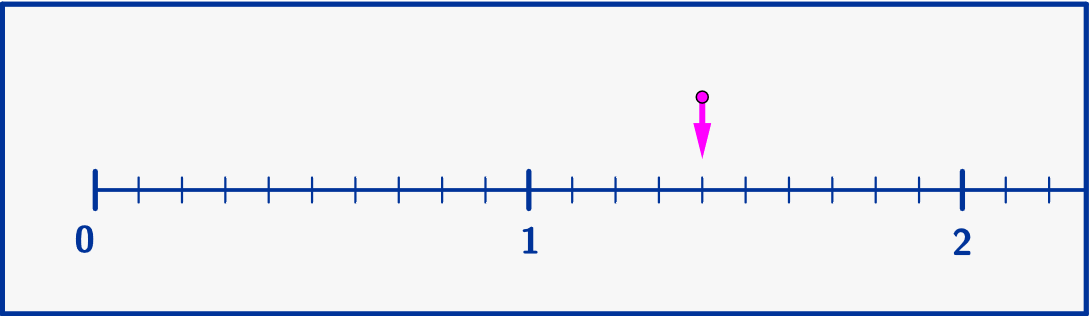
\includegraphics[width=.8\linewidth]{nombre_decimaux_demi-droite.png}
\begin{tikzpicture}[line cap=round,line join=round,>=triangle 45,x=.7cm,y=.7cm]
\clip(-7,-1.) rectangle (11.5,1.25);
\draw [line width=1.2pt,color=qqttzz] (-5.,-0.2)-- (-5.,0.2);
\draw [line width=1.2pt,color=qqttzz] (-4.3,-0.2)-- (-4.3,0.2);
\draw [line width=1.2pt,color=qqttzz] (-3.6,-0.2)-- (-3.6,0.2);
\draw [line width=1.2pt,color=qqttzz] (-2.9,-0.2)-- (-2.9,0.2);
\draw [line width=1.2pt,color=qqttzz] (-2.2,-0.2)-- (-2.2,0.2);
\draw [line width=1.2pt,color=qqttzz] (-1.5,-0.2)-- (-1.5,0.2);
\draw [line width=1.2pt,color=qqttzz] (-0.8,-0.2)-- (-0.8,0.2);
\draw [line width=1.2pt,color=qqttzz] (-0.1,-0.2)-- (-0.1,0.2);
\draw [line width=1.2pt,color=qqttzz] (0.6,-0.2)-- (0.6,0.2);
\draw [line width=1.2pt,color=qqttzz] (1.3,-0.2)-- (1.3,0.2);
\draw [line width=1.2pt,color=qqttzz] (2.,-0.2)-- (2.,0.2);
\draw [line width=1.2pt,color=qqttzz] (2.7,-0.2)-- (2.7,0.2);
\draw [line width=1.2pt,color=qqttzz] (3.4,-0.2)-- (3.4,0.2);
\draw [line width=1.2pt,color=qqttzz] (4.1,-0.2)-- (4.1,0.2);
\draw [line width=1.2pt,color=qqttzz] (4.8,-0.2)-- (4.8,0.2);
\draw [line width=1.2pt,color=qqttzz] (5.5,-0.2)-- (5.5,0.2);
\draw [line width=1.2pt,color=qqttzz] (6.2,-0.2)-- (6.2,0.2);
\draw [line width=1.2pt,color=qqttzz] (6.9,-0.2)-- (6.9,0.2);
\draw [line width=1.2pt,color=qqttzz] (7.6,-0.2)-- (7.6,0.2);
\draw [line width=1.2pt,color=qqttzz] (8.3,-0.2)-- (8.3,0.2);
\draw [line width=1.2pt,color=qqttzz] (9.,-0.2)-- (9.,0.2);
\draw [line width=1.2pt,color=qqttzz] (9.7,-0.2)-- (9.7,0.2);
\draw [line width=1.2pt,color=qqttzz] (10.4,-0.2)-- (10.4,0.2);
\draw [line width=1.8pt,color=qqttzz] (-5.,-0.3)-- (-5.,0.3);
\draw [line width=1.8pt,color=qqttzz] (2.,-0.3)-- (2.,0.3);
\draw [line width=1.8pt,color=qqttzz] (9.,-0.3)-- (9.,0.3);
\draw [->,line width=3.2pt,color=ffqqff] (0.65,1.5) -- (0.65,0.5);
\draw [line width=1.pt,color=qqttzz] (-5.1,0.)-- (11.,0.);
\draw [color=qqttzz](-5.702551640664176,-0.24500778919399624) node[anchor=north west] {$\mathbf{440}$};
\draw [color=qqttzz](1.6680669276383482,-0.29910407226410646) node[anchor=north west] {$\mathbf{450}$};
\end{tikzpicture}

\end{ExoCd} 
\end{pageParcoursd} 
 
 
\begin{pageParcourst}


\begin{ExoCt}{Chercher. Représenter.}{1234}{2}{0}{0}{0}{0}

Détermine les deux nombres entiers qui encadre le nombre donné  \vspace{0.1cm}

$$\ldots\ldots\ldots\ldots\ldots\ldots\ldots < 563\,471\,119< \ldots\ldots\ldots\ldots\ldots\ldots$$

Détermine les deux nombres entiers qui encadre le nombre donné  \vspace{0.1cm}

$$\ldots\ldots\ldots\ldots\ldots\ldots\ldots < 99\,040\,110< \ldots\ldots\ldots\ldots\ldots\ldots$$
 
\end{ExoCt}

% ExoCD 7 paramètres : Compétences, qrcode , calculatrice, python, scratch, tableur, annales
\begin{ExoCt}{Chercher. Représenter.}{1234}{2}{0}{0}{0}{0}

Ranger dans l'ordre décroissant les nombres : $ 213\,091 \quad 132\,091 \quad 123\,001 \quad 123\,901\quad 123\,109$ \vspace{0.2cm}
 \point{1} 
  \vspace{0.1cm}

Ranger dans l'ordre décroissant les nombres : $ 99\,401 \quad 99\,991 \quad 100\,001 \quad 99\,991\quad 100\,109$ \vspace{0.1cm}

 \point{1} 
 
\end{ExoCt}


\begin{ExoCt}{Chercher. Communiquer.}{1234}{2}{0}{0}{0}{0}
 
Éric a décomposé le nombre entier  $E = 23\times 1\,000\,000 + 6\times 100\,000 + 4 +  5\times 1\,000  + 4\times 100 +  2$. \vspace{0.2cm}

Peux-tu le retrouver ? $E = \ldots\ldots\ldots\ldots\ldots\ldots\ldots\ldots $
\end{ExoCt}

% ExoCT 7 paramètres : Compétences, qrcode , calculatrice, python, scratch, tableur, annales
\begin{ExoCt}{Chercher. Représenter.}{1234}{2}{0}{0}{0}{0}
 Sur la demi-droite ci-dessous :

 \begin{enumerate}[leftmargin=*]
 \item Donner les abscisses des points A, B et C.\\
 \[A(............)\hspace{1cm}B(............)\hspace{1cm}C(............)\]
 \item Placer le point D(35).
 \end{enumerate} 

 \begin{center}
     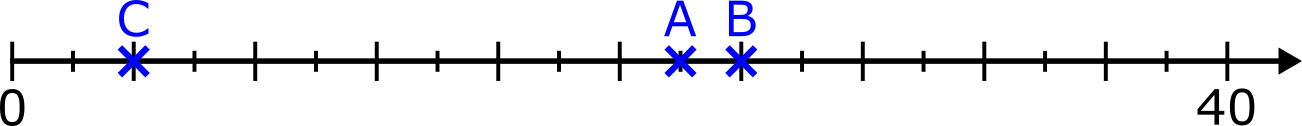
\includegraphics[width=12cm]{demi_droite.png}
 \end{center}
\end{ExoCt}
 
\begin{ExoCt}{Chercher. Représenter.}{1234}{2}{0}{0}{0}{0}
 
Cette famille est composée de nombres possédant deux propriétés.
\begin{itemize}
\item Ils s'écrivent avec 6 chiffres.
\item La somme de leurs chiffres est égale à 40.
\end{itemize}
Voici deux exemples de nombres de cette famille : 
\begin{itemize}
\item 908 878 (9+0+8+8+7+8 = 40)
\item 753 976 (7+5+3+9+7+6 = 40)
\end{itemize}
Quel est le plus petit nombre de la famille ? \point{5}

\hfill{\tiny D'après IREM Lyon}
\end{ExoCt}

\end{pageParcourst}


 
\begin{pageAuto}
% ExoCu 7 paramètres : Compétences, qrcode , calculatrice, python, scratch, tableur, annales

\begin{ExoAuto}{Chercher. Représenter.}{1234}{2}{0}{0}{0}{0}

Entoure la ou les cases justes.

\begin{tabularx}{\linewidth}{|p{6cm}|X|X|X|X|}
\hline 
Énoncé & A & B & C & D \\ 
\hline
Le nombre suivant $134\,099$ est & $134\,199$ & $134\,100$ & $135\,099$ & $135\,000$ \\ 
\hline 
$12\,407=$ & $12+407$ &  $12\times 10+407$ &  $12\times 100+407$ & $12\times 1\,000+407$ \\ 
\hline 
Dans $134\,567$, $6$ est le chiffre des & unités &  dizaines & centaines & milliers \\ 
\hline 
Le chiffres des milliers de $13\,457$ est  & $1$ & $3$ & $4$ & $5$ \\ 
\hline 
Lequel de ces nombres est compris entre $25\,340$ et $25\,350 $ & $25\,034$ & $25\,304$ & $25\,341$ & $25\,543$ \\ 
\hline 
$5\times 1\,000\,000+32\times 1\,000 +4\times 10=$ & $5\,032\,004$ &  $5\,324\,000$ &  $5\,032\,400$ &  $5\,032\,040$ \\ 
\hline 
 $134\,204$ est compris entre & $134\,203$ et $134\,205$  & $14\,203$ et $14\,205$& $134\,23$ et $134\,25$ &  $34\,203$ et $34\,205$ \\ 
\hline

\end{tabularx} 
\end{ExoAuto}

 
 

\begin{ExoAuto}{Représenter. Communiquer.}{1234}{2}{0}{0}{0}{0}

Je suis le nombre entier qui suit  $98\,045\,998$. \point{1}

Je suis le nombre entier qui précède  $25\,060\,000$. \point{1}
  
\end{ExoAuto}
 
 
\begin{ExoAuto}{Chercher.}{1234}{2}{0}{0}{0}{0}

 Le point $D$ et le point $O$ sont placés sur la droite graduée.
 
\definecolor{ffqqqq}{rgb}{1.,0.,0.}
\definecolor{wqwqwq}{rgb}{0.3764705882352941,0.3764705882352941,0.3764705882352941}
\definecolor{yqyqyq}{rgb}{0.5019607843137255,0.5019607843137255,0.5019607843137255}
\begin{tikzpicture}[line cap=round,line join=round,>=triangle 45,x=1.0cm,y=1.0cm]
\clip(1.4330456680992273,1.7995850535155078) rectangle (12.818294698183,2.4177546905415026);
\draw [color=yqyqyq](11.48969711916367,2.5) node[anchor=north west] {$541\,640$};
\draw [color=yqyqyq](1.590741496044137,2.5) node[anchor=north west] {$541\,630$};
\draw [line width=1.pt,color=wqwqwq] (2.,2.)-- (12.,2.);
\begin{scriptsize}
\draw [color=wqwqwq] (2.,2.)-- ++(-2.5pt,0 pt) -- ++(5.0pt,0 pt) ++(-2.5pt,-2.5pt) -- ++(0 pt,5.0pt);
\draw [color=wqwqwq] (3.,2.)-- ++(-2.5pt,0 pt) -- ++(5.0pt,0 pt) ++(-2.5pt,-2.5pt) -- ++(0 pt,5.0pt);
\draw [color=wqwqwq] (4.,2.)-- ++(-2.5pt,0 pt) -- ++(5.0pt,0 pt) ++(-2.5pt,-2.5pt) -- ++(0 pt,5.0pt);
\draw [color=wqwqwq] (5.,2.)-- ++(-2.5pt,0 pt) -- ++(5.0pt,0 pt) ++(-2.5pt,-2.5pt) -- ++(0 pt,5.0pt);
\draw [color=wqwqwq] (6.,2.)-- ++(-2.5pt,0 pt) -- ++(5.0pt,0 pt) ++(-2.5pt,-2.5pt) -- ++(0 pt,5.0pt);
\draw [color=wqwqwq] (7.,2.)-- ++(-2.5pt,0 pt) -- ++(5.0pt,0 pt) ++(-2.5pt,-2.5pt) -- ++(0 pt,5.0pt);
\draw [color=wqwqwq] (8.,2.)-- ++(-2.5pt,0 pt) -- ++(5.0pt,0 pt) ++(-2.5pt,-2.5pt) -- ++(0 pt,5.0pt);
\draw [color=wqwqwq] (9.,2.)-- ++(-2.5pt,0 pt) -- ++(5.0pt,0 pt) ++(-2.5pt,-2.5pt) -- ++(0 pt,5.0pt);
\draw [color=wqwqwq] (10.,2.)-- ++(-2.5pt,0 pt) -- ++(5.0pt,0 pt) ++(-2.5pt,-2.5pt) -- ++(0 pt,5.0pt);
\draw [color=wqwqwq] (11.,2.)-- ++(-2.5pt,0 pt) -- ++(5.0pt,0 pt) ++(-2.5pt,-2.5pt) -- ++(0 pt,5.0pt);
\draw [color=wqwqwq] (12.,2.)-- ++(-2.5pt,0 pt) -- ++(5.0pt,0 pt) ++(-2.5pt,-2.5pt) -- ++(0 pt,5.0pt);
\draw [color=wqwqwq] (2.5,2.)-- ++(-2.5pt,0 pt) -- ++(5.0pt,0 pt) ++(-2.5pt,-2.5pt) -- ++(0 pt,5.0pt);
\draw [color=wqwqwq] (3.5,2.)-- ++(-2.5pt,0 pt) -- ++(5.0pt,0 pt) ++(-2.5pt,-2.5pt) -- ++(0 pt,5.0pt);
\draw [color=ffqqqq] (4.5,2.)-- ++(-2.5pt,0 pt) -- ++(5.0pt,0 pt) ++(-2.5pt,-2.5pt) -- ++(0 pt,5.0pt);
\draw[color=ffqqqq] (4.561234103779965,2.2498811811635714) node {$D$};
\draw [color=wqwqwq] (5.5,2.)-- ++(-2.5pt,0 pt) -- ++(5.0pt,0 pt) ++(-2.5pt,-2.5pt) -- ++(0 pt,5.0pt);
\draw [color=wqwqwq] (6.5,2.)-- ++(-2.5pt,0 pt) -- ++(5.0pt,0 pt) ++(-2.5pt,-2.5pt) -- ++(0 pt,5.0pt);
\draw [color=wqwqwq] (7.5,2.)-- ++(-2.5pt,0 pt) -- ++(5.0pt,0 pt) ++(-2.5pt,-2.5pt) -- ++(0 pt,5.0pt);
\draw [color=wqwqwq] (8.5,2.)-- ++(-2.5pt,0 pt) -- ++(5.0pt,0 pt) ++(-2.5pt,-2.5pt) -- ++(0 pt,5.0pt);
\draw [color=ffqqqq] (9.5,2.)-- ++(-2.5pt,0 pt) -- ++(5.0pt,0 pt) ++(-2.5pt,-2.5pt) -- ++(0 pt,5.0pt);
\draw[color=ffqqqq] (9.55604435158216,2.2498811811635714) node {$O$};
\draw [color=wqwqwq] (10.5,2.)-- ++(-2.5pt,0 pt) -- ++(5.0pt,0 pt) ++(-2.5pt,-2.5pt) -- ++(0 pt,5.0pt);
\draw [color=wqwqwq] (11.5,2.)-- ++(-2.5pt,0 pt) -- ++(5.0pt,0 pt) ++(-2.5pt,-2.5pt) -- ++(0 pt,5.0pt);
\end{scriptsize}
\end{tikzpicture}

\vspace{0.2cm}

 Le point $D$ a pour abscisse $\ldots\ldots\ldots\ldots\ldots\ldots$ et le point $O$ a pour abscisse $\ldots\ldots\ldots\ldots\ldots\ldots$.
 
\end{ExoAuto}
 
\begin{ExoAuto}{Chercher. Communiquer.}{1234}{2}{0}{0}{0}{0}

 Place sur la droite graduée le point A d'abscisse $235\,645$
 \vspace{0.2cm}
 
\definecolor{wqwqwq}{rgb}{0.3764705882352941,0.3764705882352941,0.3764705882352941}
\definecolor{yqyqyq}{rgb}{0.5019607843137255,0.5019607843137255,0.5019607843137255}
\begin{tikzpicture}[line cap=round,line join=round,>=triangle 45,x=1.0cm,y=1.0cm]
\clip(1.408318884694266,1.7171624352453752) rectangle (12.310052437048013,2.434239214195529);
\draw [color=yqyqyq](11.08969711916367,2.5 ) node[anchor=north west] {$235\,650$};
\draw [color=yqyqyq](1.490741496044137,2.5) node[anchor=north west] {$235\,640$};
\draw [line width=1.pt,color=wqwqwq] (2.,2.)-- (12.,2.);
\begin{scriptsize}
\draw [line width=1.6pt,color=yqyqyq] (2.,2.)-- ++(-2.5pt,0 pt) -- ++(5.0pt,0 pt) ++(-2.5pt,-2.5pt) -- ++(0 pt,5.0pt);
\draw [color=wqwqwq] (3.,2.)-- ++(-2.5pt,0 pt) -- ++(5.0pt,0 pt) ++(-2.5pt,-2.5pt) -- ++(0 pt,5.0pt);
\draw [color=wqwqwq] (4.,2.)-- ++(-2.5pt,0 pt) -- ++(5.0pt,0 pt) ++(-2.5pt,-2.5pt) -- ++(0 pt,5.0pt);
\draw [color=wqwqwq] (5.,2.)-- ++(-2.5pt,0 pt) -- ++(5.0pt,0 pt) ++(-2.5pt,-2.5pt) -- ++(0 pt,5.0pt);
\draw [color=wqwqwq] (6.,2.)-- ++(-2.5pt,0 pt) -- ++(5.0pt,0 pt) ++(-2.5pt,-2.5pt) -- ++(0 pt,5.0pt);
\draw [color=wqwqwq] (7.,2.)-- ++(-2.5pt,0 pt) -- ++(5.0pt,0 pt) ++(-2.5pt,-2.5pt) -- ++(0 pt,5.0pt);
\draw [color=wqwqwq] (8.,2.)-- ++(-2.5pt,0 pt) -- ++(5.0pt,0 pt) ++(-2.5pt,-2.5pt) -- ++(0 pt,5.0pt);
\draw [color=wqwqwq] (9.,2.)-- ++(-2.5pt,0 pt) -- ++(5.0pt,0 pt) ++(-2.5pt,-2.5pt) -- ++(0 pt,5.0pt);
\draw [color=wqwqwq] (10.,2.)-- ++(-2.5pt,0 pt) -- ++(5.0pt,0 pt) ++(-2.5pt,-2.5pt) -- ++(0 pt,5.0pt);
\draw [color=wqwqwq] (11.,2.)-- ++(-2.5pt,0 pt) -- ++(5.0pt,0 pt) ++(-2.5pt,-2.5pt) -- ++(0 pt,5.0pt);
\draw [line width=1.6pt,color=yqyqyq] (12.,2.)-- ++(-2.5pt,0 pt) -- ++(5.0pt,0 pt) ++(-2.5pt,-2.5pt) -- ++(0 pt,5.0pt);
\draw [color=wqwqwq] (2.5,2.)-- ++(-2.5pt,0 pt) -- ++(5.0pt,0 pt) ++(-2.5pt,-2.5pt) -- ++(0 pt,5.0pt);
\draw [color=wqwqwq] (3.5,2.)-- ++(-2.5pt,0 pt) -- ++(5.0pt,0 pt) ++(-2.5pt,-2.5pt) -- ++(0 pt,5.0pt);
\draw [color=wqwqwq] (4.5,2.)-- ++(-2.5pt,0 pt) -- ++(5.0pt,0 pt) ++(-2.5pt,-2.5pt) -- ++(0 pt,5.0pt);
\draw [color=wqwqwq] (5.5,2.)-- ++(-2.5pt,0 pt) -- ++(5.0pt,0 pt) ++(-2.5pt,-2.5pt) -- ++(0 pt,5.0pt);
\draw [color=wqwqwq] (6.5,2.)-- ++(-2.5pt,0 pt) -- ++(5.0pt,0 pt) ++(-2.5pt,-2.5pt) -- ++(0 pt,5.0pt);
\draw [color=wqwqwq] (7.5,2.)-- ++(-2.5pt,0 pt) -- ++(5.0pt,0 pt) ++(-2.5pt,-2.5pt) -- ++(0 pt,5.0pt);
\draw [color=wqwqwq] (8.5,2.)-- ++(-2.5pt,0 pt) -- ++(5.0pt,0 pt) ++(-2.5pt,-2.5pt) -- ++(0 pt,5.0pt);
\draw [color=wqwqwq] (9.5,2.)-- ++(-2.5pt,0 pt) -- ++(5.0pt,0 pt) ++(-2.5pt,-2.5pt) -- ++(0 pt,5.0pt);
\draw [color=wqwqwq] (10.5,2.)-- ++(-2.5pt,0 pt) -- ++(5.0pt,0 pt) ++(-2.5pt,-2.5pt) -- ++(0 pt,5.0pt);
\draw [color=wqwqwq] (11.5,2.)-- ++(-2.5pt,0 pt) -- ++(5.0pt,0 pt) ++(-2.5pt,-2.5pt) -- ++(0 pt,5.0pt);
\end{scriptsize}
\end{tikzpicture}
\end{ExoAuto}
 
 


\end{pageAuto}
